\documentclass[11pt,a4paper]{article}

% package importing
%\usepackage[margin=2cm]{geometry}
\usepackage{geometry}
 \geometry{
 a4paper,
 %total={170mm,257mm},
 left=20mm,
 top=20mm,
 right=20mm,
 bottom=20mm,
 }
 		%$$$$$$ fonts settings $$$$$$%
%\usepackage[sc]{mathpazo}  %for palatino font
%\usepackage{eulervm}  %for Euler maths font

		%$$$$$$ package imports $$$$$$%
\usepackage{amsmath}  %for mathematics
\usepackage{titlesec}  %for title spacing only
\usepackage{lipsum}  %random huge text generation
\usepackage{titlesec} %for changing font of titles 
\usepackage{amssymb}  %for real number set symbol
\usepackage{amsthm}  %for mathematics package
\usepackage{mathtools}  %for floor and ceiling
\usepackage{algorithmicx}  %for dynamic algorithm
\usepackage{algorithm}  %algorithm micro
\usepackage{algpseudocode}  %pseudocode commands
\usepackage{wrapfig}  %for wrapping figures around text
\usepackage{multicol}  %for multiple columns floats
\usepackage{enumitem}  %for enumerate numbering
\usepackage{url}   %for writing the url
\usepackage{color}  %for colorred text
\usepackage{tcolorbox}  %for colour box highlighting
\usepackage{listings}  %for code listing

% $$$$$$$$$ new command and theorems self-defined
\theoremstyle{definition}
\newtheorem{theorem}{Theorem}[section]
\newtheorem{corollary}{Corollary}[theorem]
\newtheorem{lemma}[theorem]{Lemma}
\newtheorem*{remark}{Remark}
\newtheorem{definition}{Definition}[section]
\newtheorem{example}{Example}[section]
\newtheorem{notation}{Notation}[section]
\newtheorem{algoalgorithm}{Algorithm}[section]
\newtheorem{method}{Method}[section]

% $$$$$$$$ set general info $$$$$$$
\title{\textsl{National University of Singapore} \\ \textbf{CS2106 Operating System}\\ Second Half Summary Notes}
\author{\textit{Dong Shaocong} A0148008J}

% $$$$$$$$ package parameter setting $$$$$$$$$

% for title spacing {left}{before}{after}  ----------------------------
\titlespacing\section{0.5pt}{10pt plus 2pt minus 2pt}{2pt plus 2pt minus 1pt}
\titlespacing\subsection{0.5pt}{10pt plus 2pt minus 2pt}{2pt plus 2pt minus 1pt}
\titlespacing\subsubsection{0.5pt}{10pt plus 2pt minus 2pt}{2pt plus 2pt minus 1pt}

% for title font specifications  ------------------------------------------
\titleformat{\section}
  {\normalfont\fontsize{16}{16}\bfseries}
  {\thesection}{1em}{}
  
\titleformat{\subsection}
  {\normalfont\fontsize{14}{14}\bfseries}{\thesection}{1em}{}
  
\titleformat{\subsubsection}
  {\normalfont\fontsize{13}{13}\bfseries}{\thesection}{1em}{}

% declare floor and ceiling functions   ------------------------------------------
\DeclarePairedDelimiter\ceil{\lceil}{\rceil}
\DeclarePairedDelimiter\floor{\lfloor}{\rfloor}

% set the numbering of enumerate to numbers------------------------------------------
\setlist[enumerate]{label*=\arabic*.}
%\setlist{nolistsep}
\newenvironment{myitemize}
{ \begin{itemize}
    \setlength{\itemsep}{5pt}
    \setlength{\parskip}{0pt}
    \setlength{\parsep}{0pt}     }
{ \end{itemize}                  } 
\newenvironment{myenumerate}
{ \begin{enumerate}
    \setlength{\itemsep}{5pt}
    \setlength{\parskip}{0pt}
    \setlength{\parsep}{0pt}     }
{ \end{enumerate}                } 

% $$$$$$$$$ math symbols cheatsheet
% Caligraphic letters: $\mathcal{A}$ 
% Mathbb letters: $\mathbb{A}$
% Mathfrak letters: $\mathfrak{A}$ 
% Math Sans serif letters: $\mathsf{A}$ 
% $$$$$ color text commands ------------
\newcommand{\redtt}[1]{{\color{red}\texttt{#1}}}
\newcommand{\bluett}[1]{{\color{blue}\texttt{#1}}}
\newcommand{\browntt}[1]{{\color{brown}\texttt{#1}}}
\newcommand{\bluebf}[1]{{\color{blue} \huge \textbf{#1}}}
\renewcommand{\emph}[2]{\redtt{#1} \bluebf{#2}}
%-------------------------------------------------------

% $$$$$$$$ start of documents $$$$$$$$$
\begin{document}
\maketitle
\section{File System}

\begin{definition}{\textbf{File system}}
	\begin{myitemize}
		\item Present logical (abstract) view of files and directories
		\begin{myitemize}
			\item Accessing a disk is very complicated: (2D or 3D structure, track/surface/sector, seek, rotation, $\dots$)
			\item Hide complexity of hardware devices
		\end{myitemize}
		\item Facilitate efficient use of storage devices: Optimise access e.g. to disk.
		\item Support sharing
		\begin{myitemize}
			\item Files persist even when owner/creator is not currently active (unlike main memory)
			\item Key issue: Provide protection (control access)
		\end{myitemize}
	\end{myitemize}
\end{definition}

\begin{definition}{\textbf{Hierarchical View of File system}}
	\begin{center}
		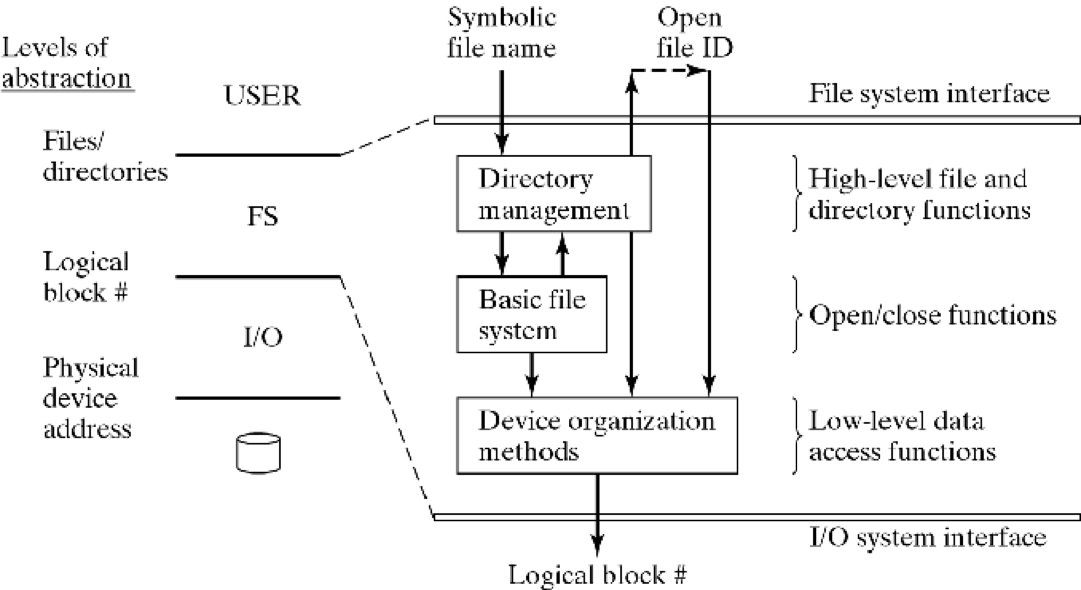
\includegraphics[scale=0.5]{m2/hierarchyFileSystem}
	\end{center}
	\begin{myitemize}
		\item \textbf{Directory management}: map logical name to
unique Id, file descriptor
		\item \textbf{Basic file system}: open/close files
		\item \textbf{Physical device  organization}: map file data to disk blocks
	\end{myitemize}
\end{definition}

\begin{definition}{\textbf{User-end view of File}}
	\begin{myitemize}
		\item \textbf{File name and type}
		\begin{myitemize}
			\item Valid name: number or characters, lower or upper cases, illegal characters $\dots$
			\item Extension: tied to type of file, used by applications
			\item File type is recorded in header
			\begin{myitemize}
				\item Cannot be changed (even when extension changes)
				\item Basic types: text, object, load file, directory
				\item Application-specific types, e.g., .doc, .ps, .html
			\end{myitemize}
		\end{myitemize}
		\item \textbf{Logical file organization}
		\begin{myitemize}
			\item Most common: byte stream
			\item Fixed-size or variable-size records
			\item Addressed: \textbf{Implicitly} (sequential access to next record), or \textbf{Explicitly} by position (record\#) or key
			\begin{center}
				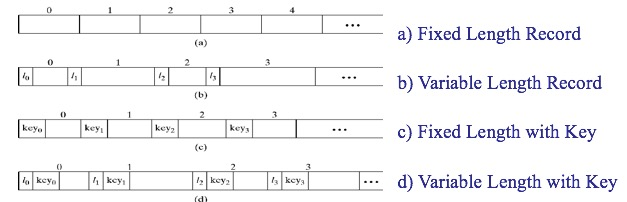
\includegraphics[scale=0.4]{m2/fileOrgType}
			\end{center}
		\end{myitemize}
	\end{myitemize}
\end{definition}

\begin{definition}{\textbf{Directory Management}}
\begin{myitemize}
	\item \textbf{Main issues}:
	\begin{myitemize}
		\item \textbf{Shape} of the data structure
		\item \textbf{What} info to keep about files
		\item \textbf{Where} to keep the files in directory
		\item \textbf{How} to organise entries for efficiency?
	\end{myitemize}
	\item \textbf{File directory data structure}:
	\begin{myitemize}
		\item \textbf{Tree-structured}
		\begin{myitemize}
			\item \textbf{Simple} search, insert, delete operations
			\item Sharing is \textbf{asymmetric}
			\begin{center}
				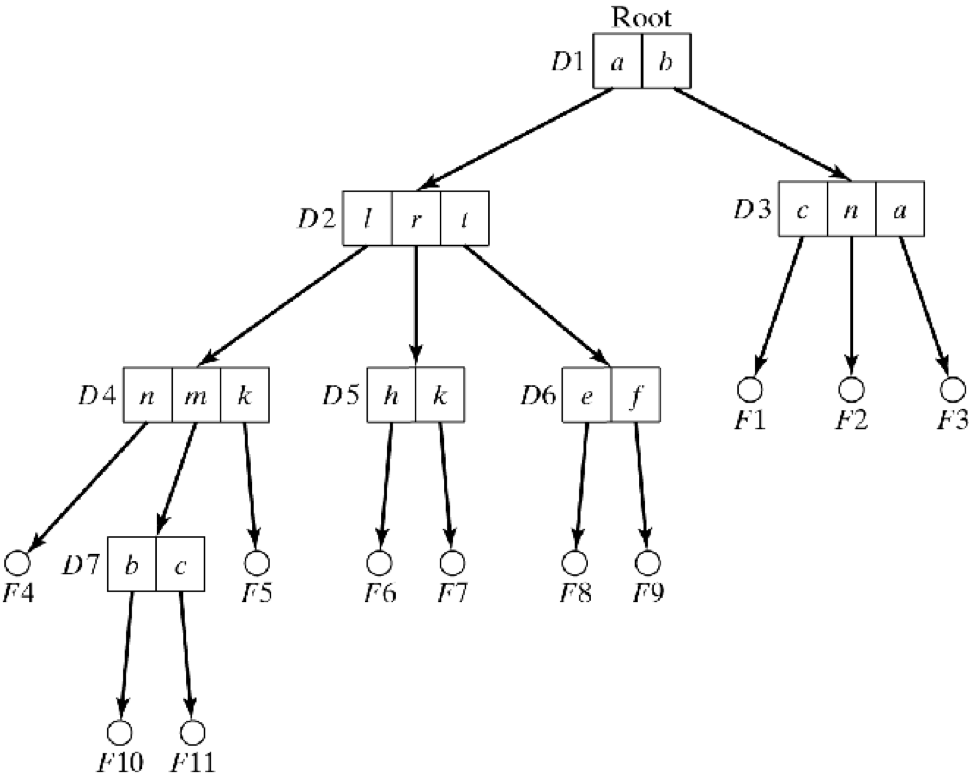
\includegraphics[scale=0.3]{m2/treeStructureFile}
			\end{center}
		\end{myitemize}
		\item \textbf{DAG-structured}
		\begin{myitemize}
			\item \textbf{Symmetric} sharing
			\item \textbf{Delete}: only last parent should remove files, so need \textbf{Reference count}
			\begin{center}
				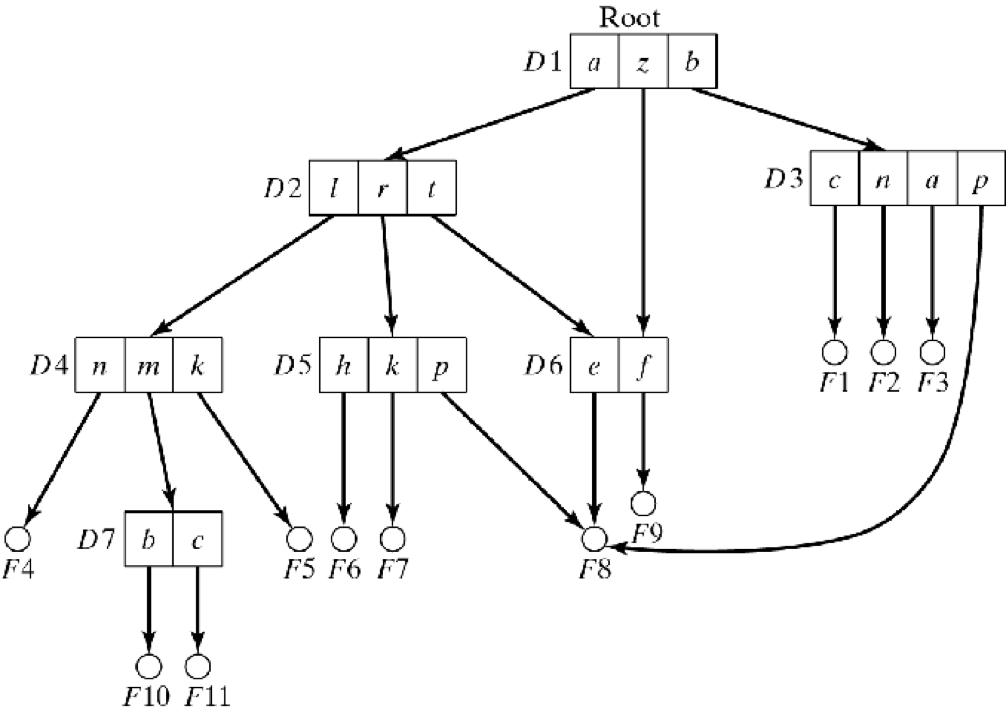
\includegraphics[scale=0.3]{m2/DAGStructureFile}
			\end{center}
		\end{myitemize}
		\item \textbf{DAG-structured with cycles}
		\begin{myitemize}
			\item Search is difficult with infinite loops
			\item Deletion needs \textbf{garbage collection} (reference count not enough)
		\end{myitemize}
		\begin{center}
			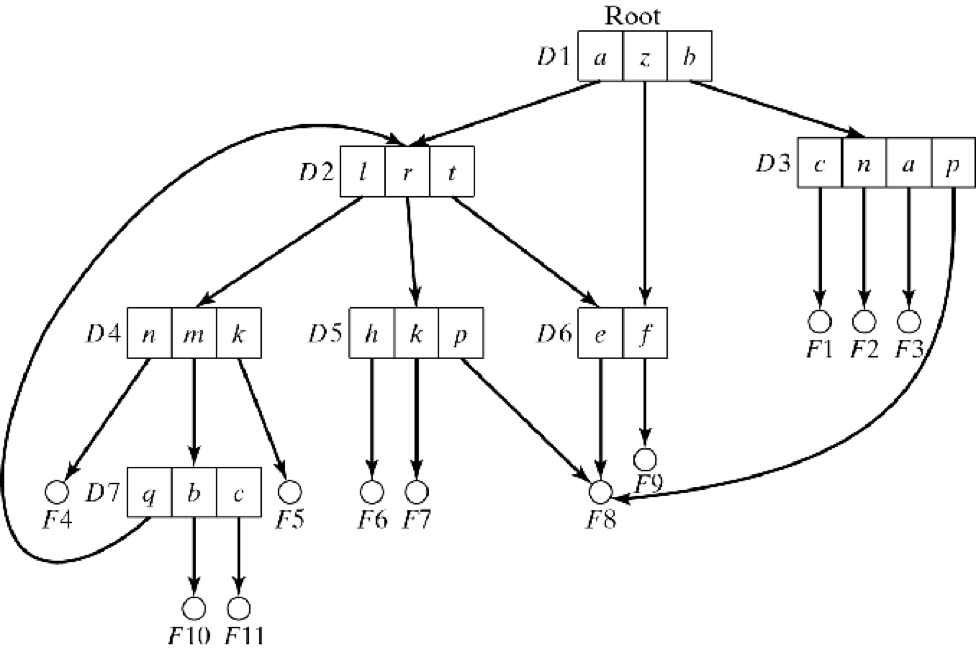
\includegraphics[scale=0.3]{m2/DAGwithCycleFile}
		\end{center}
		\item \textbf{Symbolic links (shortcuts)}
		\begin{myitemize}
			\item \textbf{Compromise} to allow sharing but avoid cycles.
			\item For \textbf{read/write}: symbolic link is the same as actual link.
			\item For \textbf{deletion}: only symbolic link is deleted.
		\end{myitemize}
		\begin{center}
			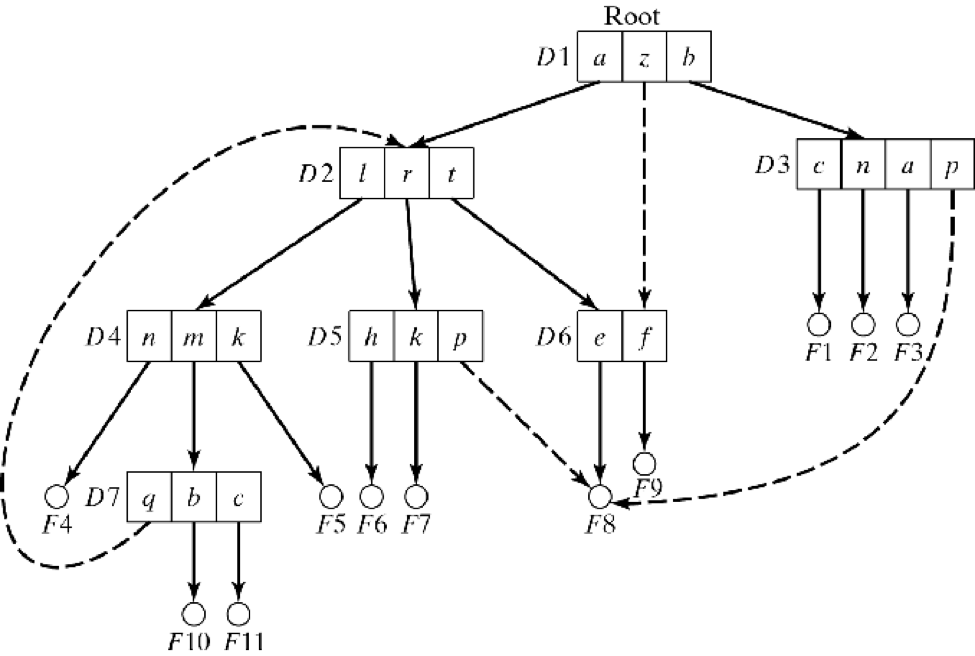
\includegraphics[scale=0.3]{m2/symbolicStructureFile}
		\end{center}
	\end{myitemize}
\end{myitemize}
\end{definition}

\begin{definition}{\textbf{UNIX Hard Links}}
	\vspace{3mm}
	
	\hspace{-15mm}
	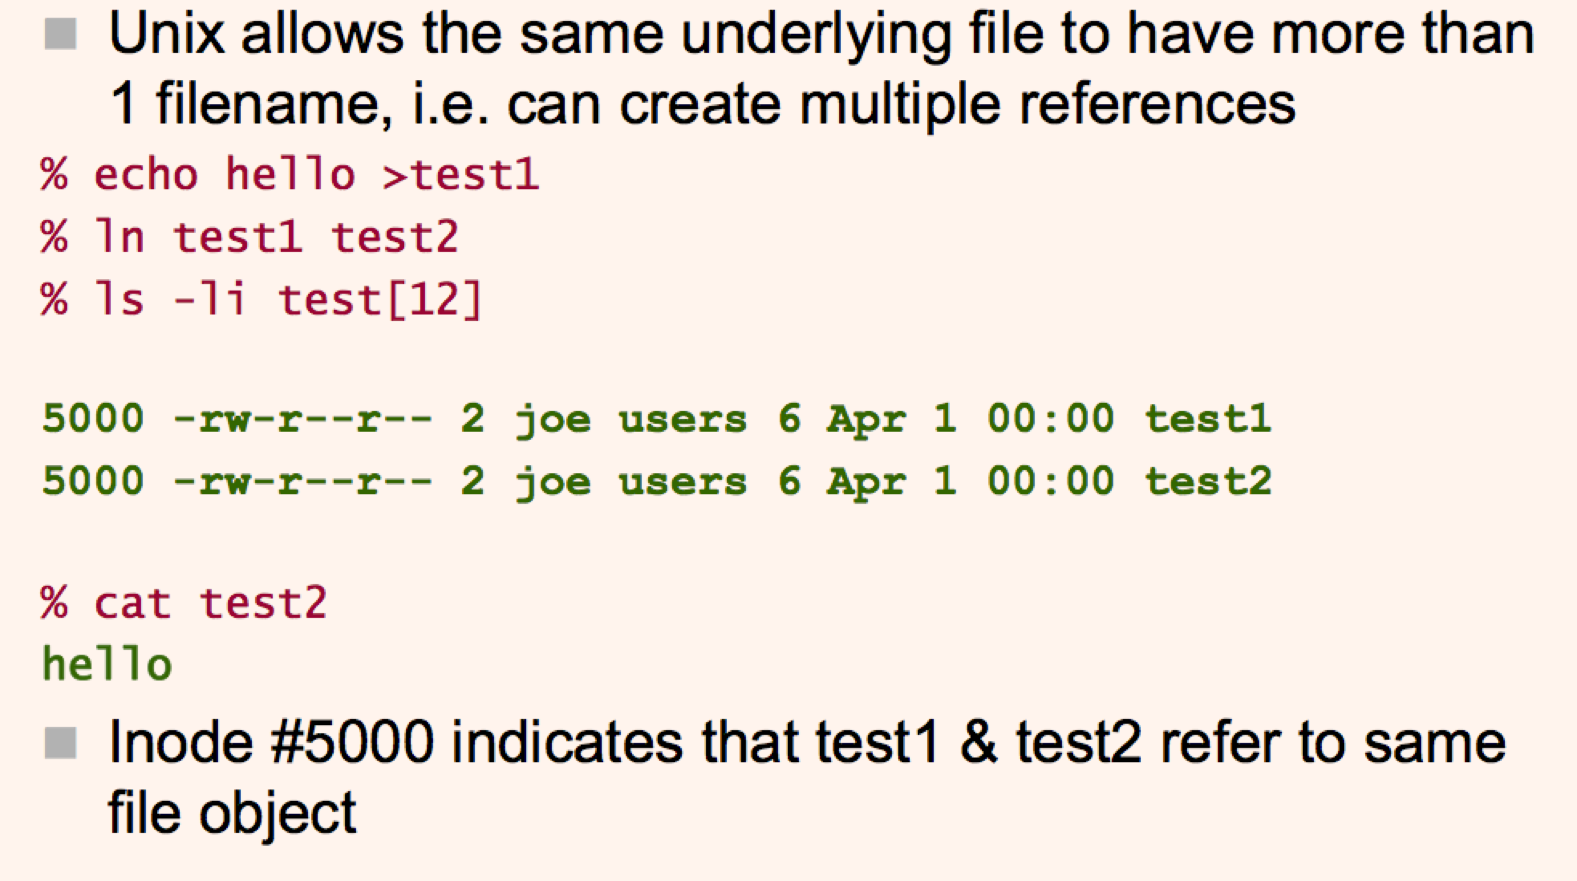
\includegraphics[scale=0.35]{m2/unixHardLink1}
	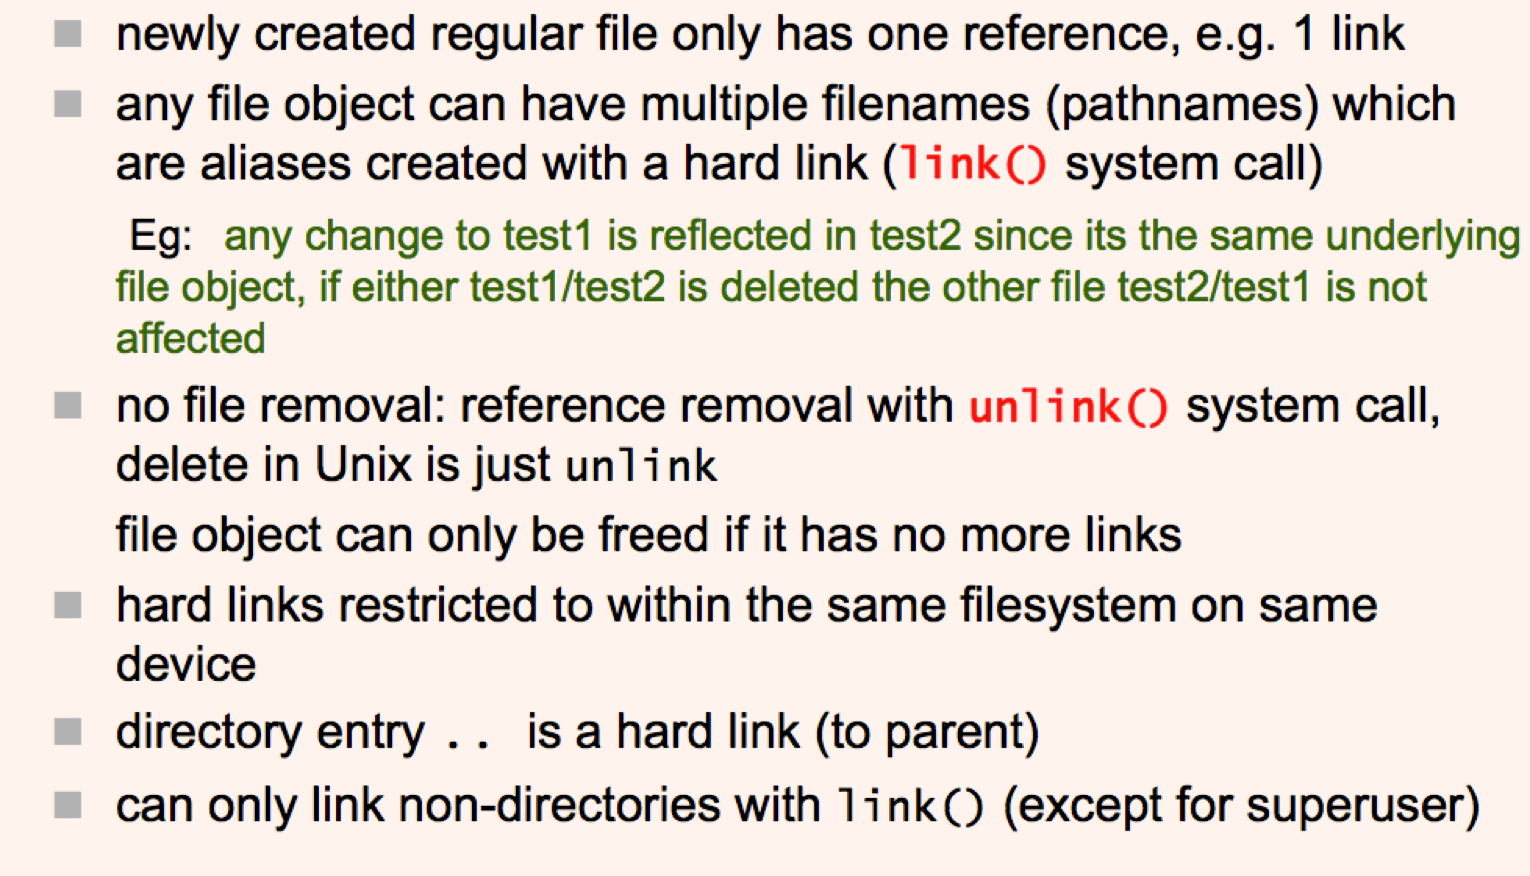
\includegraphics[scale=0.35]{m2/unixHardLink2}
	
\end{definition}

\begin{definition}{\textbf{Symbolic Links}}
	\vspace{3mm}
	
	\hspace{-15mm}
	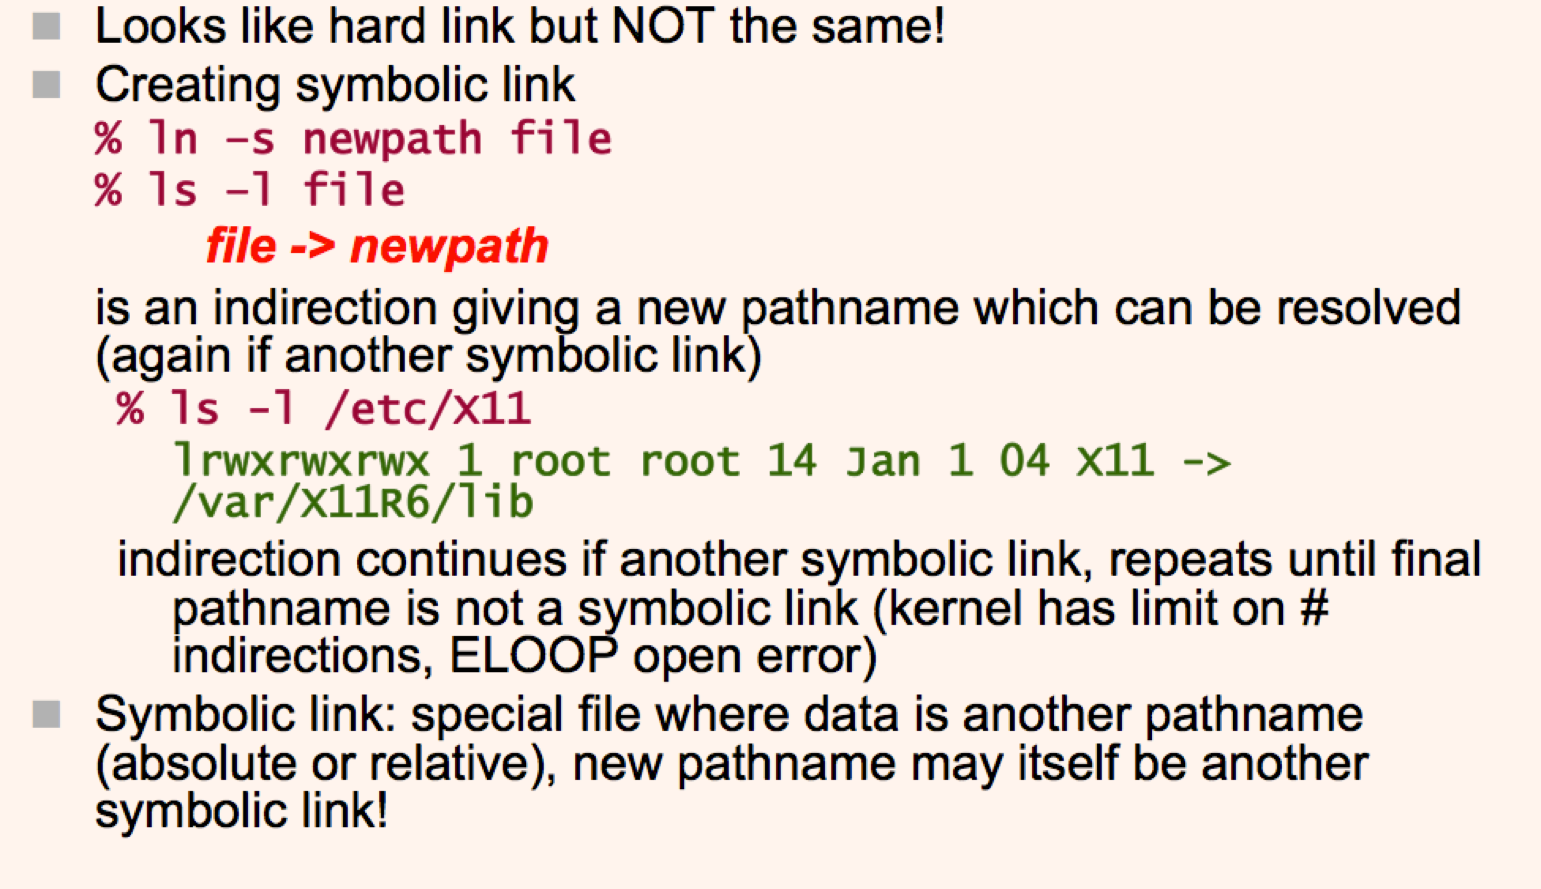
\includegraphics[scale=0.36]{m2/symbolicLink1}
	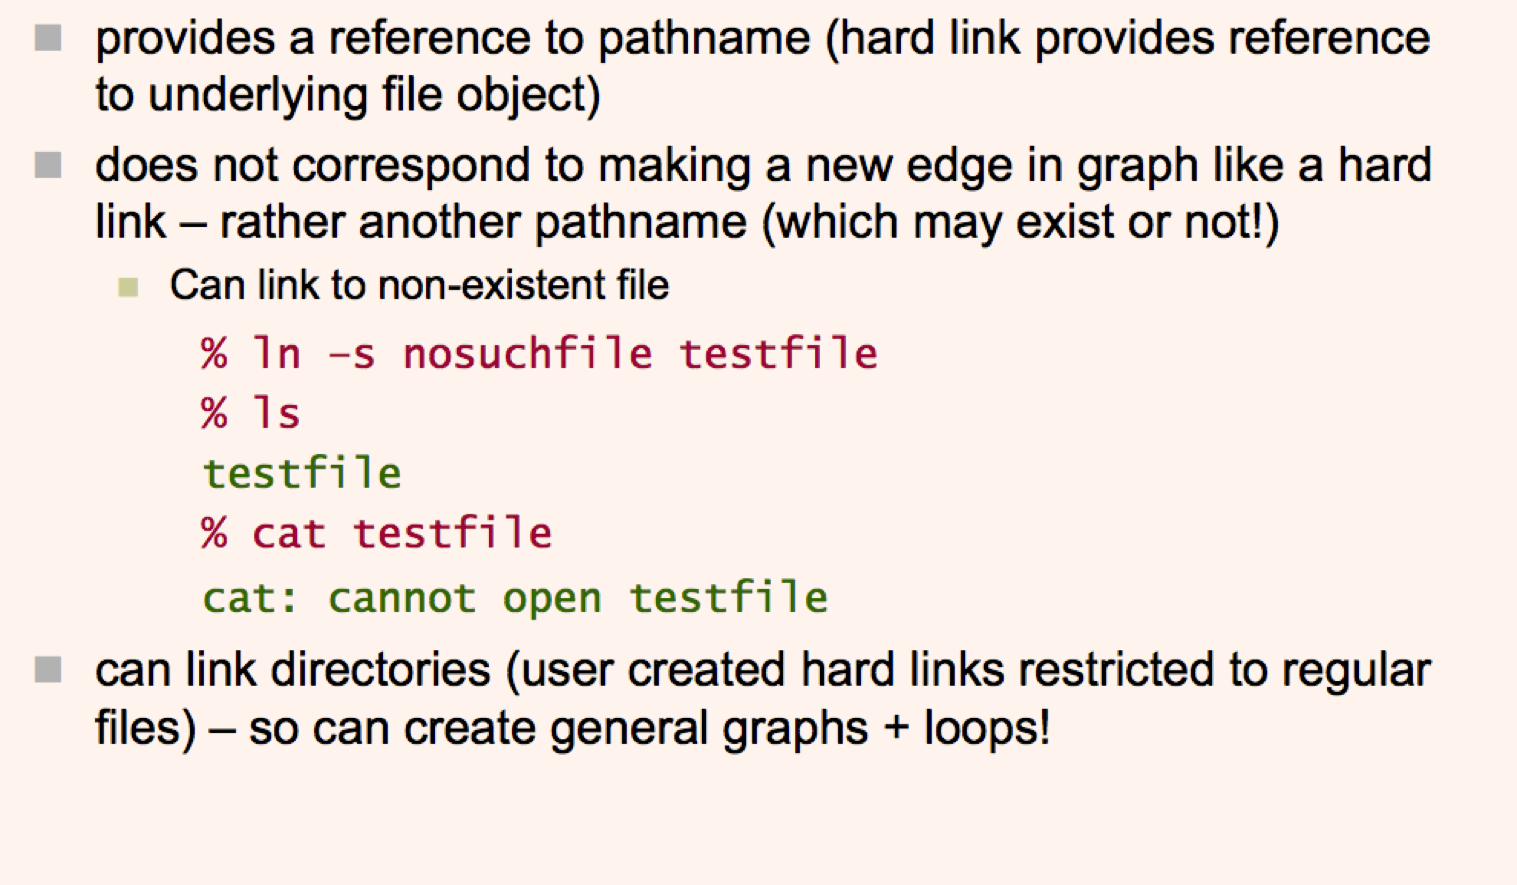
\includegraphics[scale=0.36]{m2/symbolicLink2}
	
\end{definition}

\begin{remark}{\textbf{Windows Shortcuts}}
	\begin{myitemize}
		\item Similar to symbolic links but does not re-expand further
		\item Only understood by GUI shell! Created also from GUI shell
		\item Win NTFS has hard links, symbolic links using junction mechanism (not normally used)
	\end{myitemize}
\end{remark}

\begin{remark}{\textbf{File Directories - Path name}}
	\begin{myitemize}
		\item Concatenated local names with delimiter (. or / or $\backslash$ )
		\item \textbf{Absolute} path name: start with root (/)
		\item \textbf{Relative} path name: start with current directory (.)
		\item Notation to move upward in hierarchy (..)
	\end{myitemize}
\end{remark}

\begin{minipage}{0.45\linewidth}
	\begin{method}{\textbf{Implementation of Directories}}
		\begin{myitemize} 
		\item \textbf{What information to keep in each entry}
		\begin{myitemize}
			\item \textbf{All} descriptive information, directory can become very large, searches are difficult / slow.
			\item Only symbolic \textbf{name and pointer} to descriptor
			\begin{myitemize}
				\item Needs an extra disk access to descriptor
				\item Variable name length
			\end{myitemize}
		\end{myitemize}
		\item \textbf{How to organise entries within directory}
		\begin{myitemize}
			\item \textbf{Fixed-size} entries: use array of slots
			\item \textbf{Variable-size} entries: use linked list
			\item \textbf{Size of directory}: fixed or expanding
		\end{myitemize}
	\end{myitemize}
	\end{method}
	\end{minipage}\hspace{5mm}
	\begin{minipage}{0.5\linewidth}
		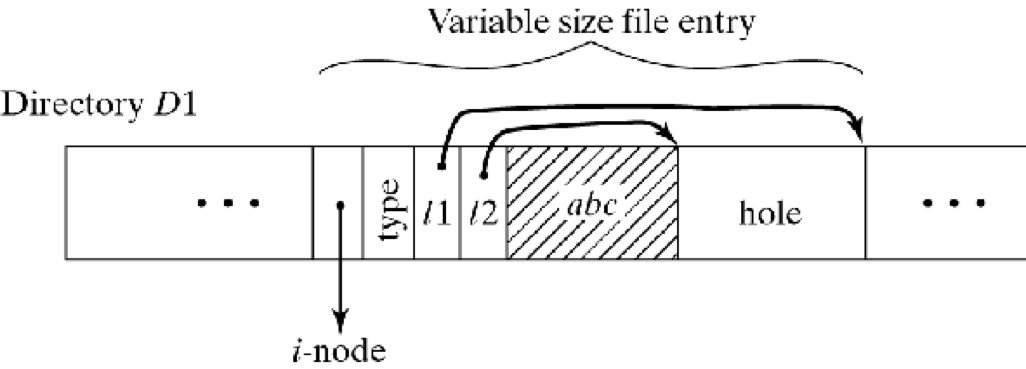
\includegraphics[width=0.8\linewidth ]{m2/implementDirectory}
		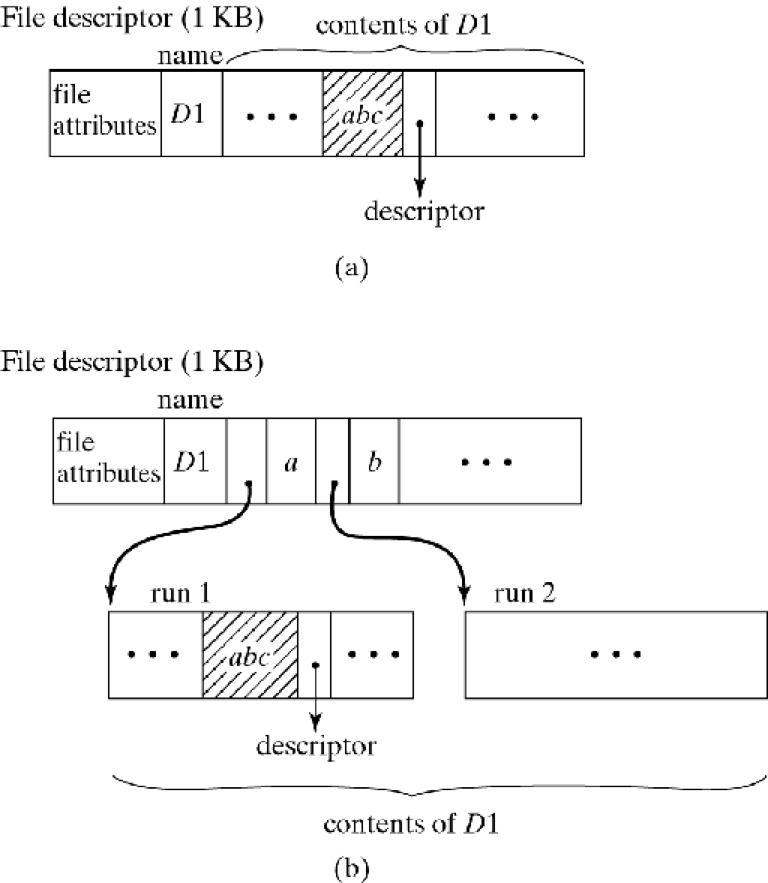
\includegraphics[width=0.8\linewidth ]{m2/entryOrganization}
	\end{minipage}
	
\begin{definition}{\textbf{File Descriptor}}
	Owner id; File type; Protection information; Mapping to physical disk blocks; Time of creation, last use, last modification; Reference counter.
\end{definition}

\begin{definition}{\textbf{OFT - Open file table}}
	keeps track of currently open files. \textbf{OFT entries}: current position; information from descriptor (file length, disk location); pointers to allocated buffers.
\end{definition}

\begin{definition}{\textbf{Basic File System Operations}}
	\begin{myitemize}
		\item \textbf{\textsf{open} file}
		\begin{myenumerate}
			\item Search directory for given file and verify access rights
			\item Allocate and fill in OFT entries and read/write buffers
			\item Return OFT index
		\end{myenumerate}
		\item \textbf{\textsf{close} command}
		\begin{myenumerate}
			\item Flush modified buffers to disk and release buffers
			\item Update file descriptor (file length, disk location, usage information)
			\item Free OFT entry
		\end{myenumerate}
		\item \textbf{\textsf{read} command}: assume file is open for \textbf{sequential} access
		\begin{myitemize}
			\item \textbf{Buffered read}: current block kept in r/w buffer
			\begin{myenumerate}
				\item copy from buffer to memory until desired count or end of file is reached: - update current position, return status
				\item copy from buffer to memory until end of buffer is reached: write the buffer to disk if modified; read the next block; continue copying
			\end{myenumerate}
			\item \textbf{Unbuffered read}: read the entire block containing the needed data from disk
		\end{myitemize}
		\item \textbf{\textsf{write} command (buffered)}
		\begin{myenumerate}
			\item Write into buffer,
			\item When full, write buffer to disk. If next block does not exist (file is expanding): - allocate new block -update file descriptor - update bit map (free space on disk).
			\item Update file length in descriptor
		\end{myenumerate}
		\item \textbf{\textsf{seek} command}
		\begin{myenumerate}
			\item Set current position as specified by parameter
			\item Read block containing current position into buffer
		\end{myenumerate}
		\item \textbf{\textsf{rewind} command}: analogous to seek but position is zero
	\end{myitemize}
\end{definition}
	
\begin{definition}{\textbf{Organising data on a disk}}

	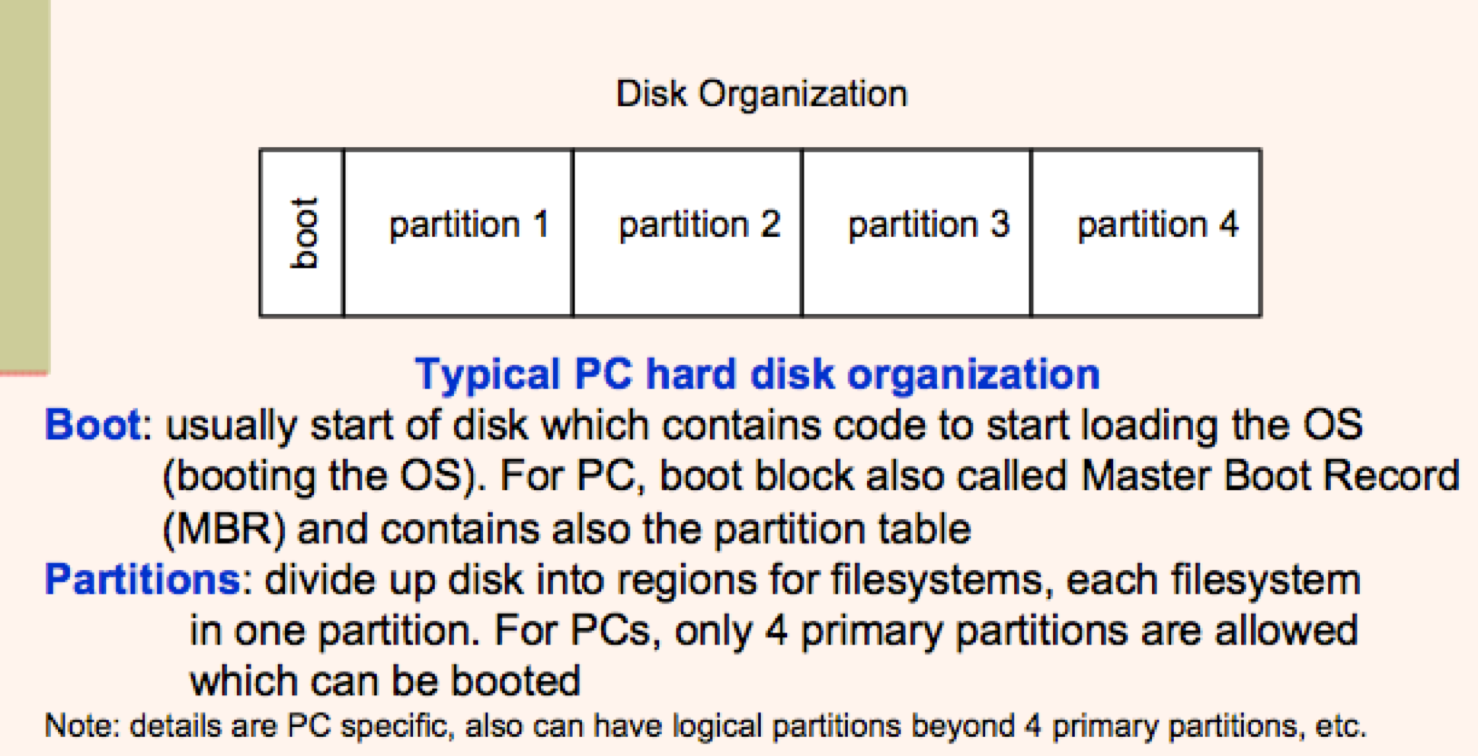
\includegraphics[width=0.48\linewidth]{m2/diskOrgnization1}
	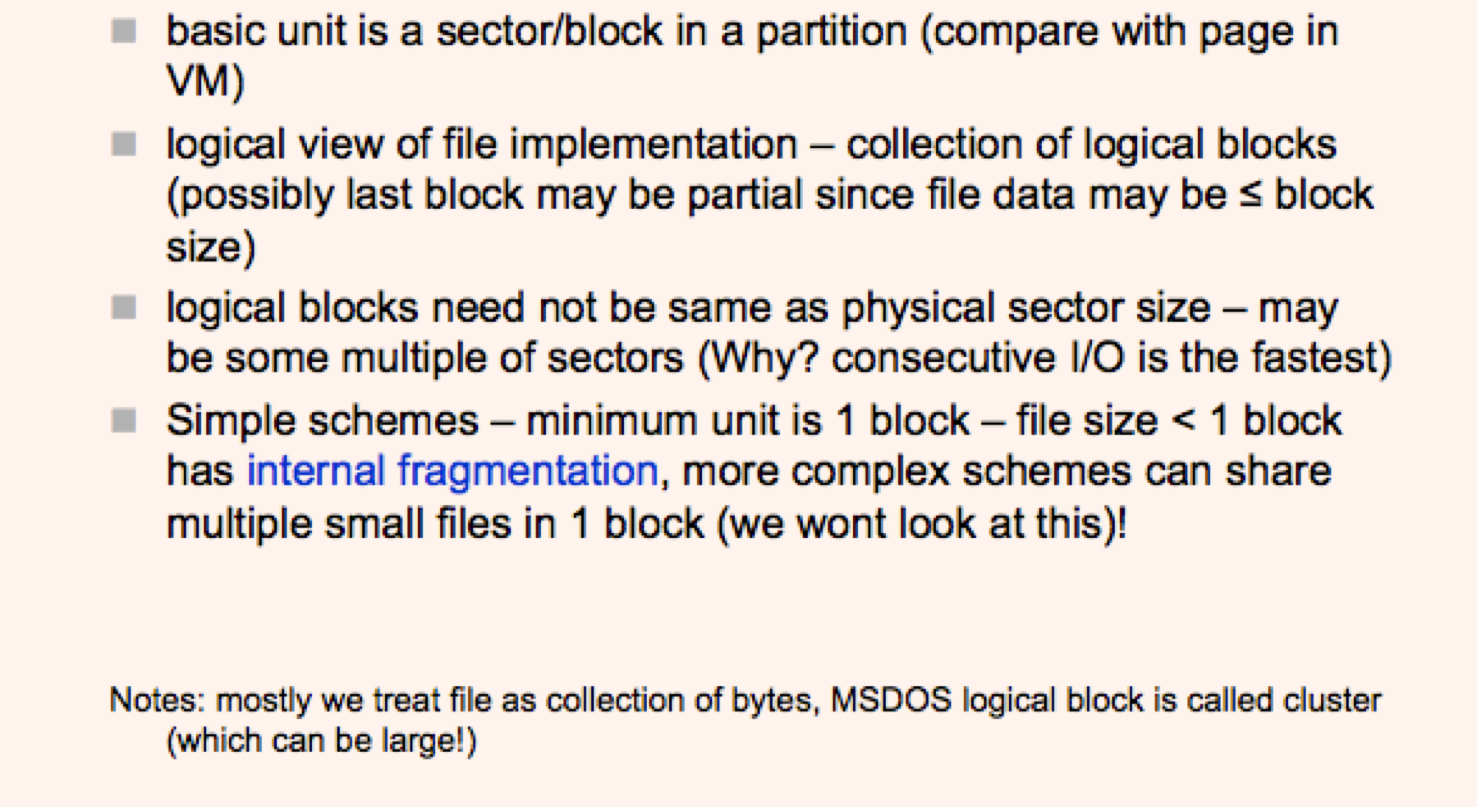
\includegraphics[width=0.48\linewidth]{m2/diskOrgnization2}
\end{definition}

\begin{definition}{\textbf{Fragmentation}}
	\begin{myitemize}
		\item \textbf{Internal fragmentation}: Due to the rules governing memory allocation, more computer memory is sometimes allocated than is needed. Any process, no matter how small, occupies an entire partition. This waste is called internal fragmentation. (unused memory within the allocated region)
		\item \textbf{External fragmentation}: External fragmentation arises when free memory is separated into small blocks and is interspersed by allocated memory. (unusable storage is outside the allocated regions.)
	\end{myitemize}
\end{definition}
	
\begin{definition}{\textbf{Data structures on Disk}}
	\textbf{Note}: need to record which block belongs to which part of files. Data structure must also be stored on disk.
	\begin{myitemize}
		\item \textbf{Contiguous organization}
		\begin{myenumerate}
			\item \textbf{Advantages}: Simple implementation; Fast sequential access (minimal arm movement)
			\item \textbf{Disadvantages}: Insert/delete is difficult; How much space to allocate initially? External fragmentation

			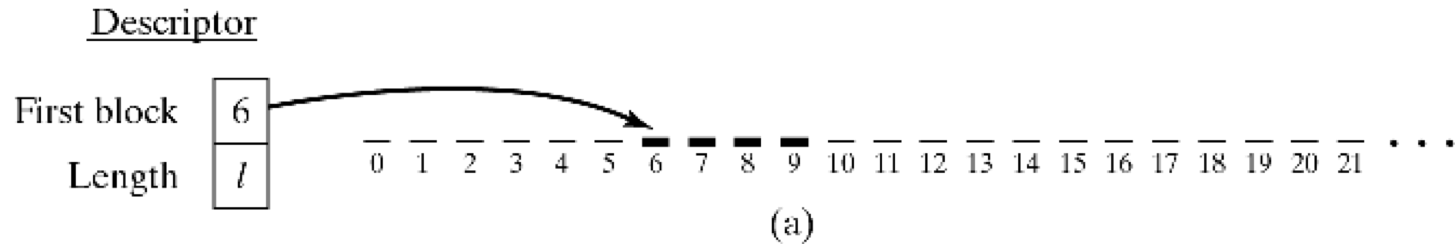
\includegraphics[width=1.0\linewidth]{m2/contiguousOrganization}
		\end{myenumerate}
		\item \textbf{Linked organization}
		\begin{myenumerate}
			\item \textbf{Advantages}: Simple insert/delete, no external fragmentation
			\item \textbf{Disadvantages}: Sequential access less efficient (seek latency); Direct access not possible; Poor reliability (when chain breaks)

			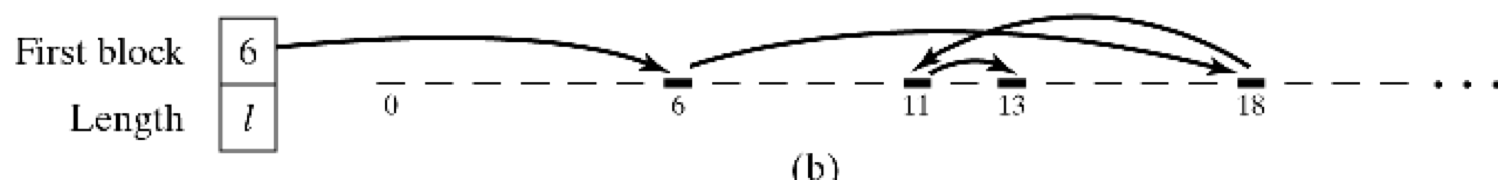
\includegraphics[width=1.0\linewidth]{m2/linkedOrganization}
			
			\item \textbf{Linked Variation 1}: keep pointers segregated, may be cached.

			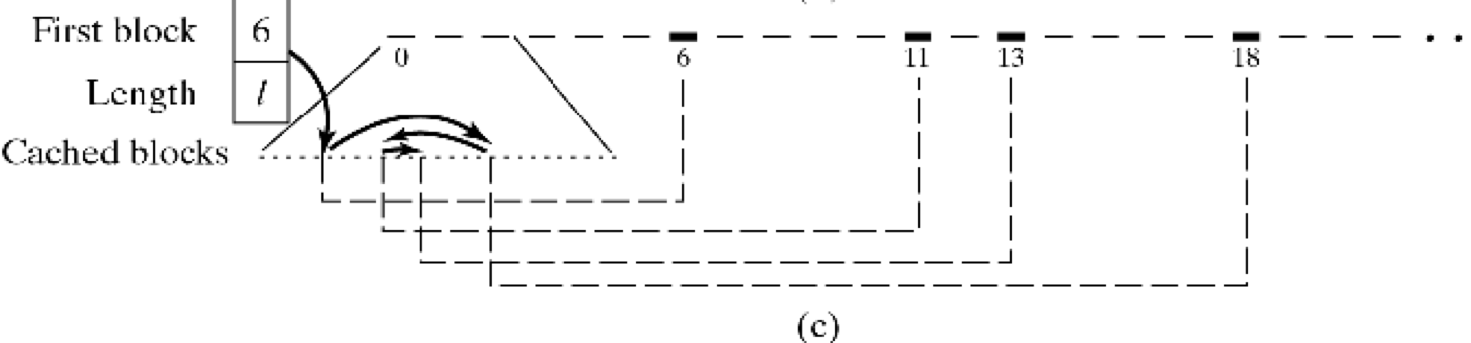
\includegraphics[width=1.0\linewidth]{m2/linkedVariation1}
			
			\item \textbf{Linked Variation 2}: Link sequences of adjacent blocks, rather than individual blocks 
			
			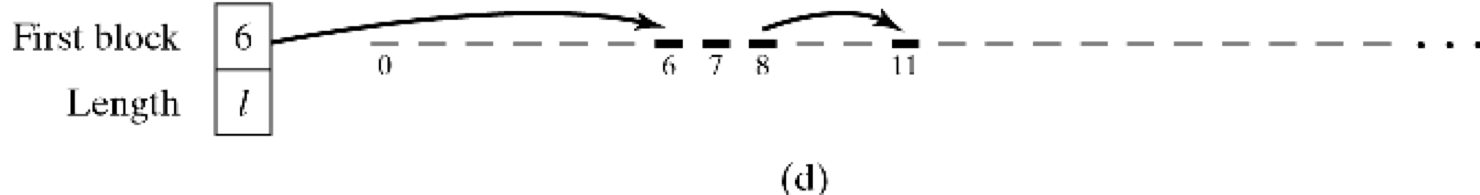
\includegraphics[width=1.0\linewidth]{m2/linkedVariation2}
			
			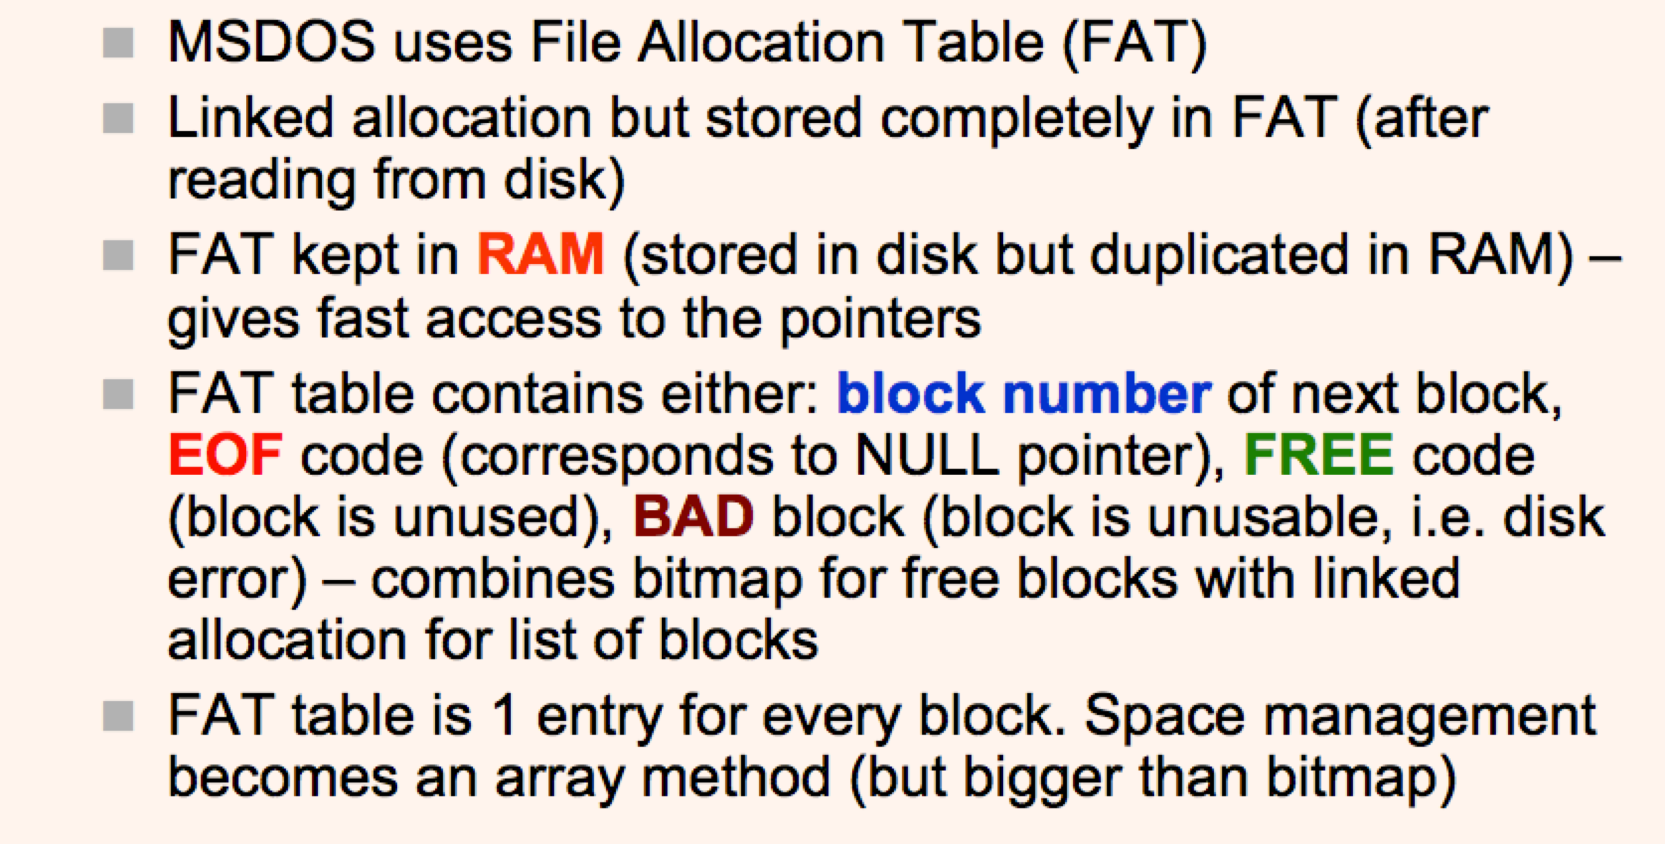
\includegraphics[width=0.50\linewidth]{m2/MSDOSFAT1}
			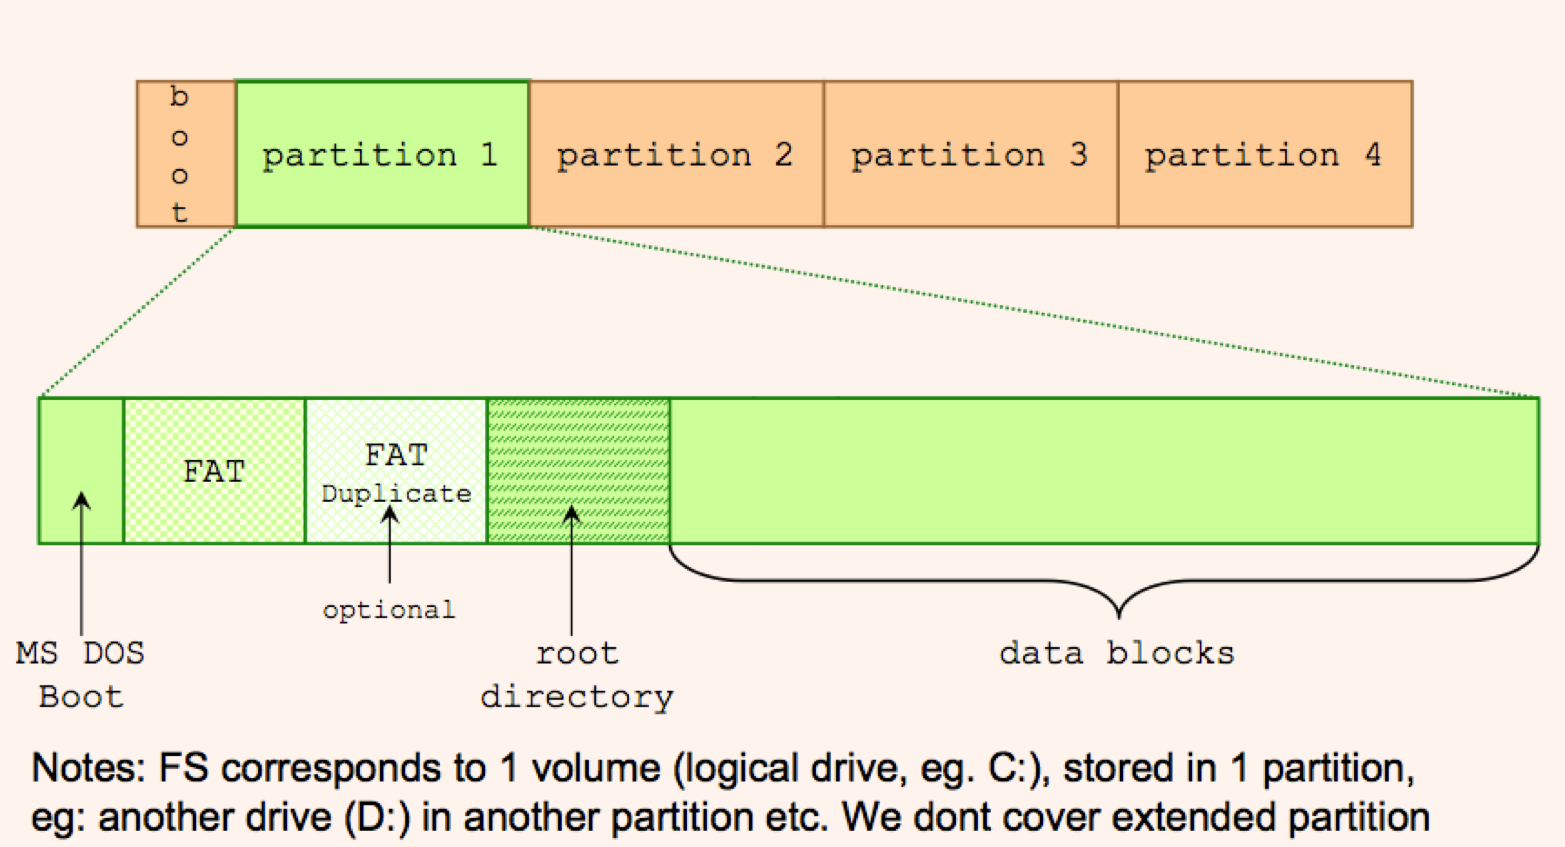
\includegraphics[width=0.50\linewidth]{m2/MSDOSFAT2}
			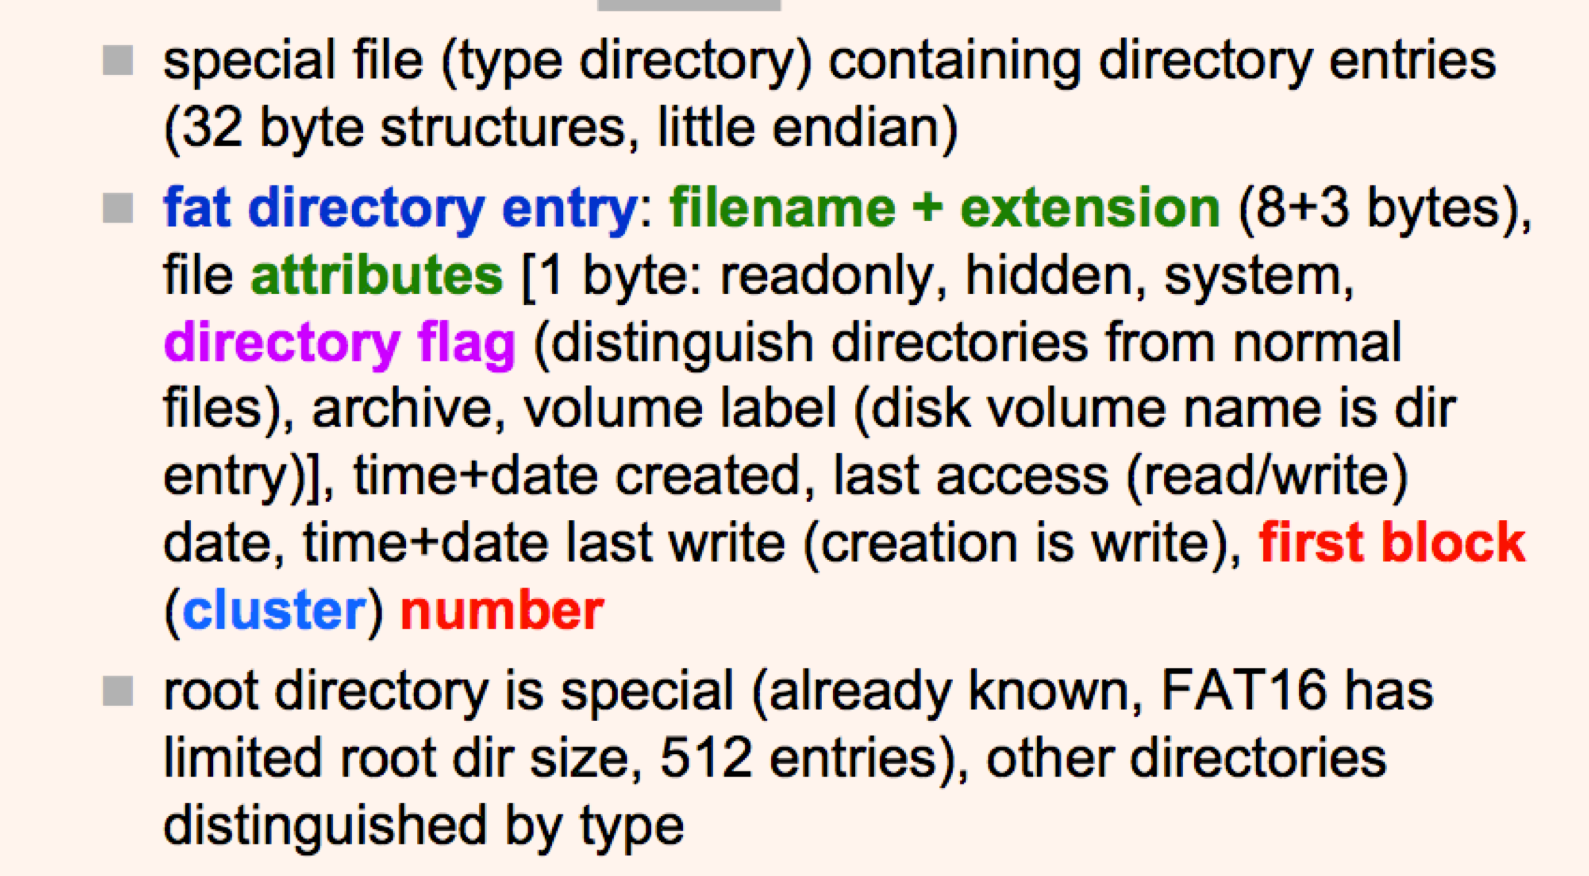
\includegraphics[width=0.50\linewidth]{m2/MSDOSFAT3}
			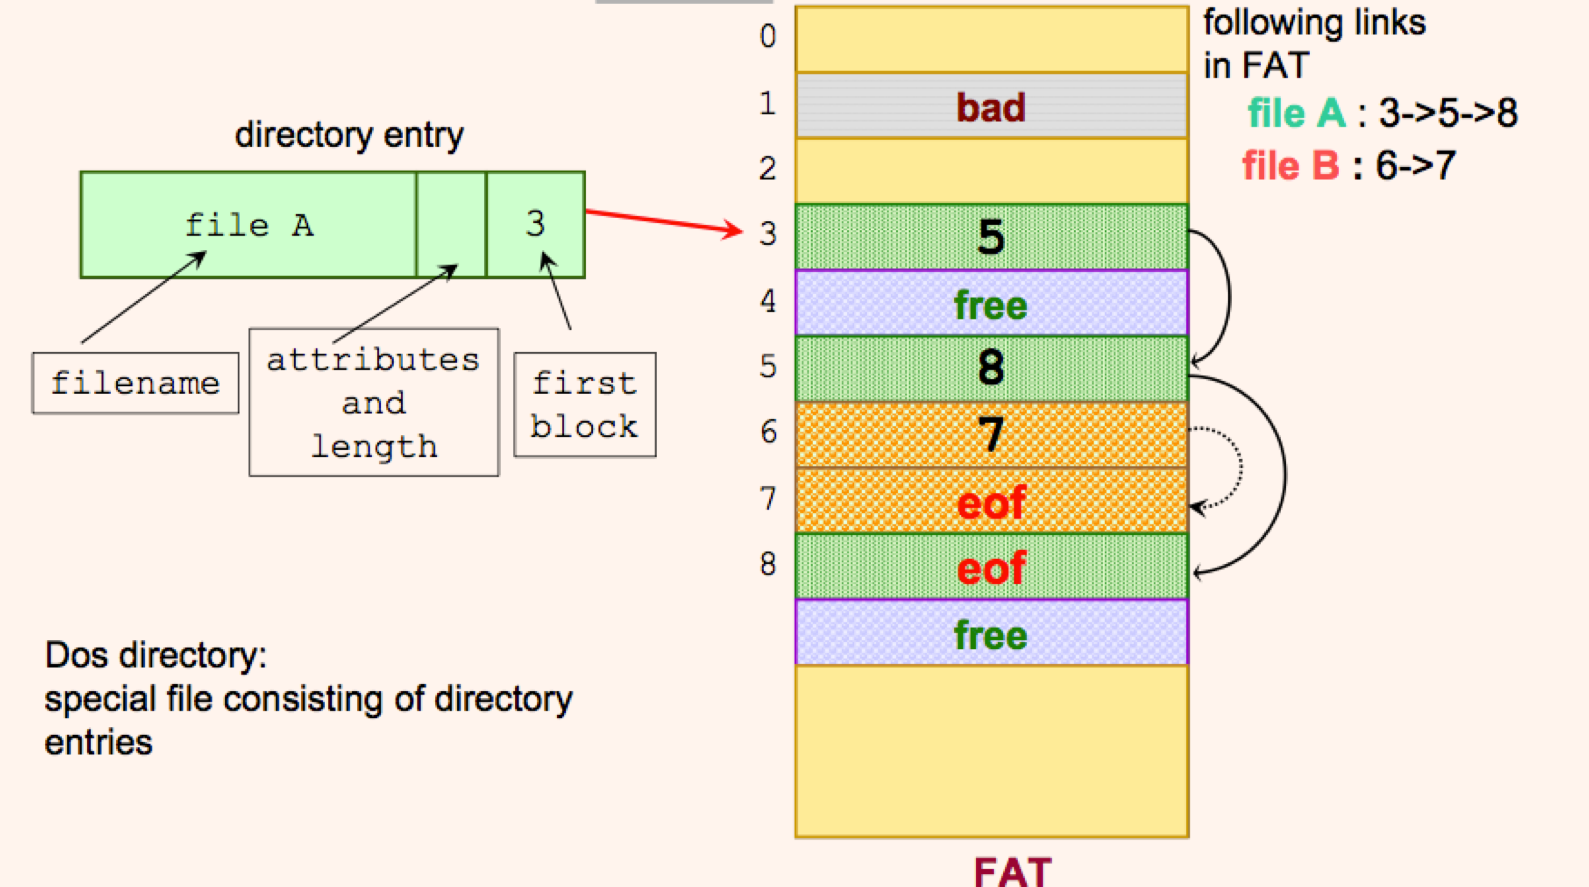
\includegraphics[width=0.50\linewidth]{m2/MSDOSFAT4}
			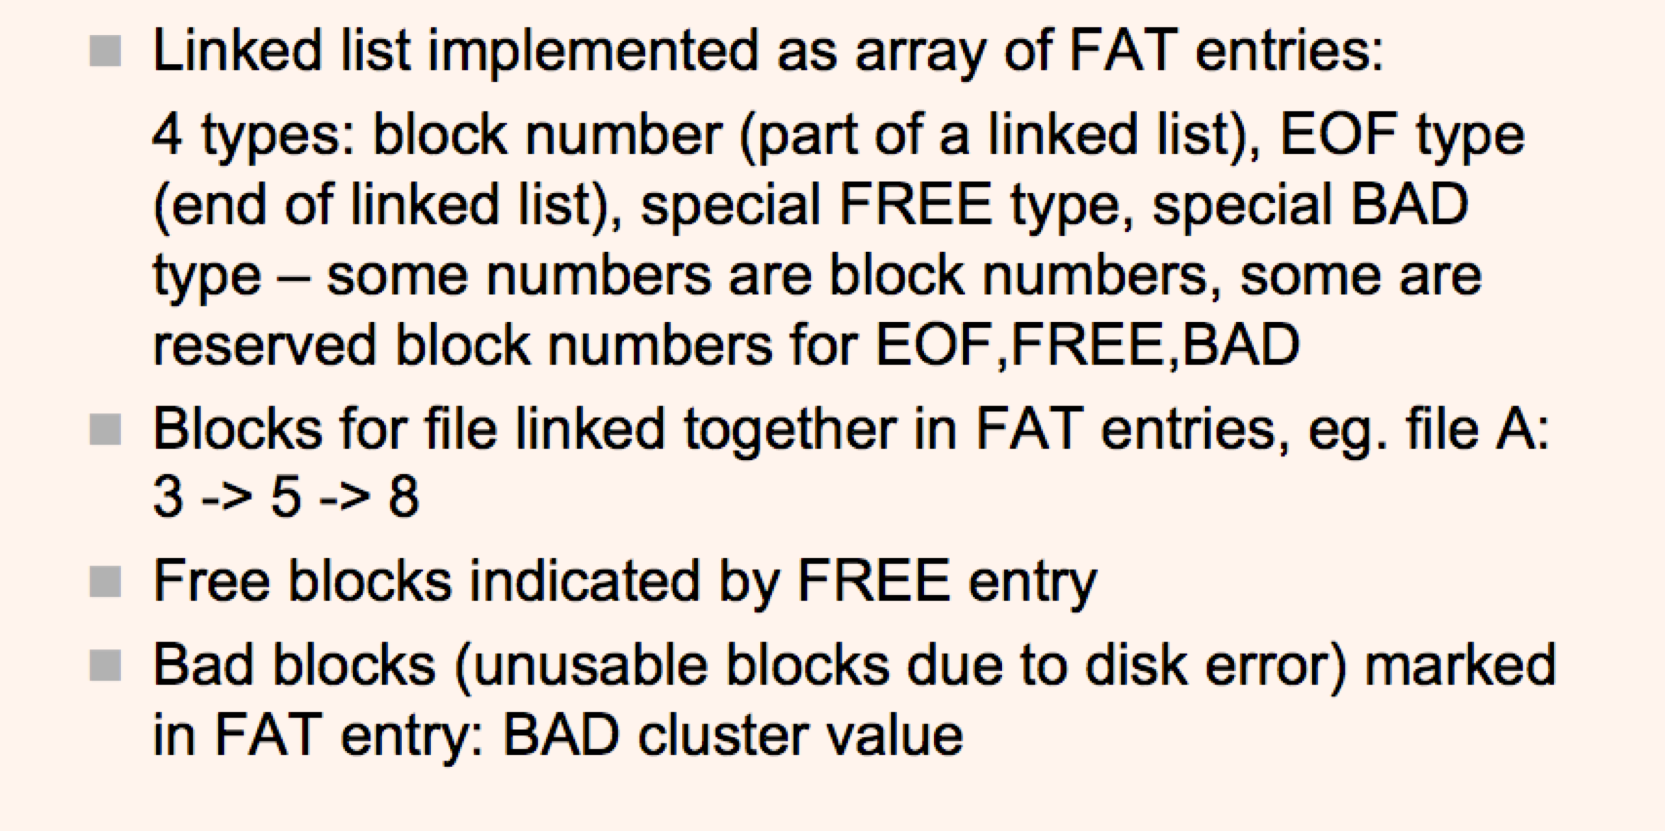
\includegraphics[width=0.50\linewidth]{m2/MSDOSFAT5}
			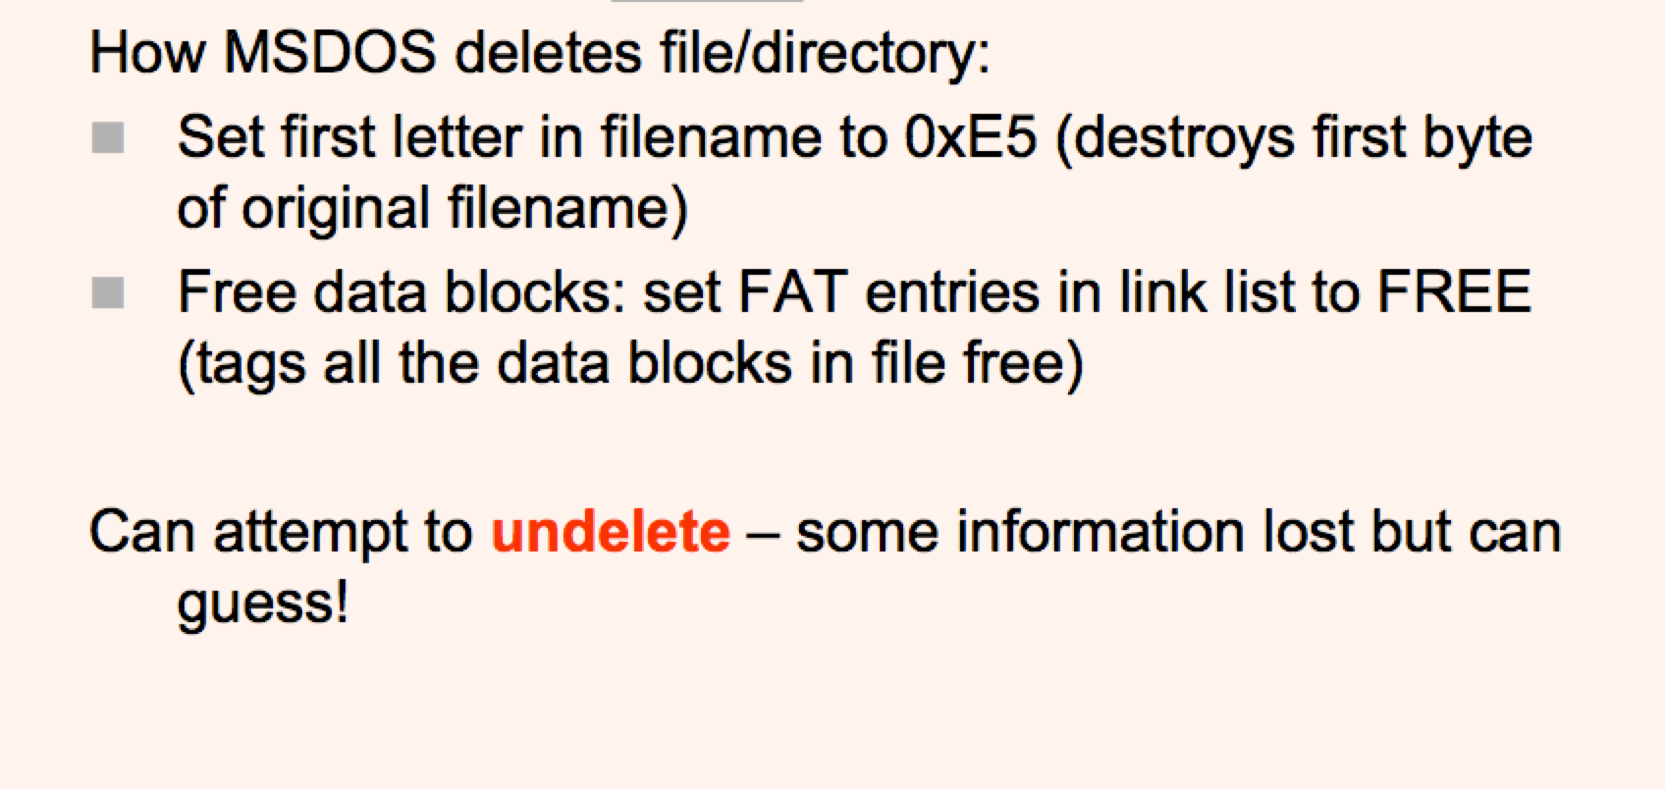
\includegraphics[width=0.50\linewidth]{m2/MSDOSFAT6}
			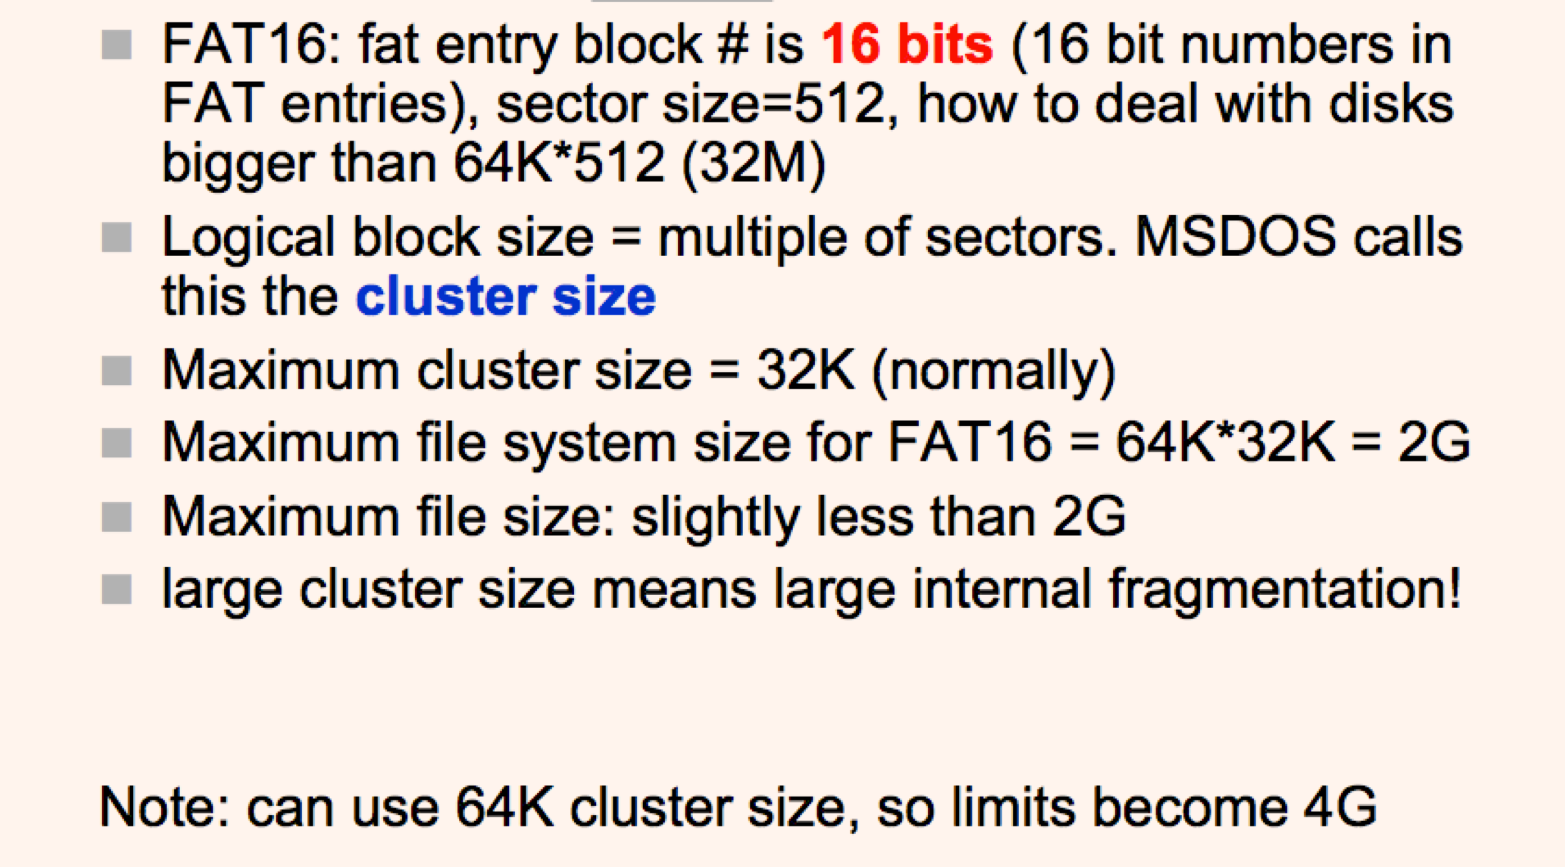
\includegraphics[width=0.50\linewidth]{m2/MSDOSFAT7}
			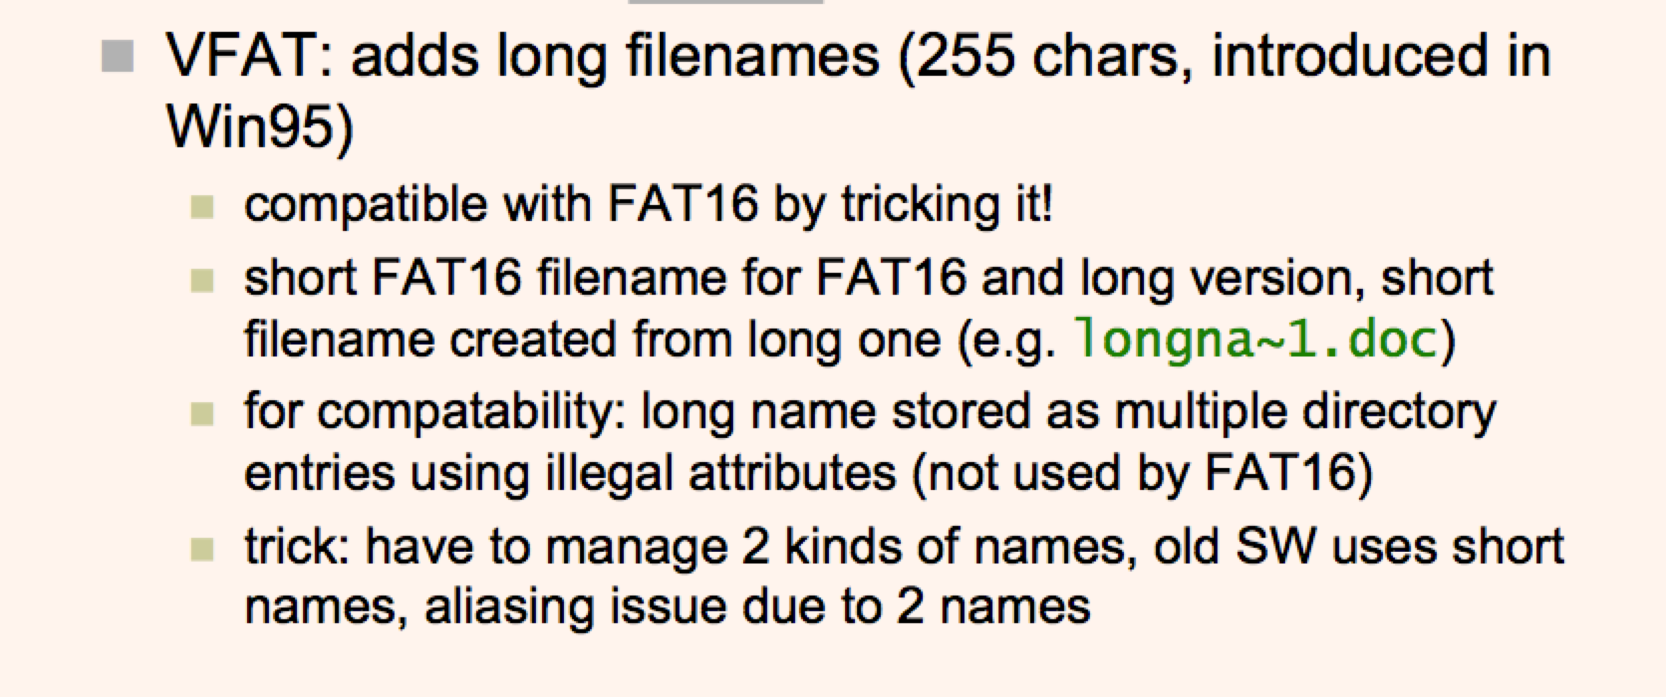
\includegraphics[width=0.50\linewidth]{m2/MSDOSFAT8}
			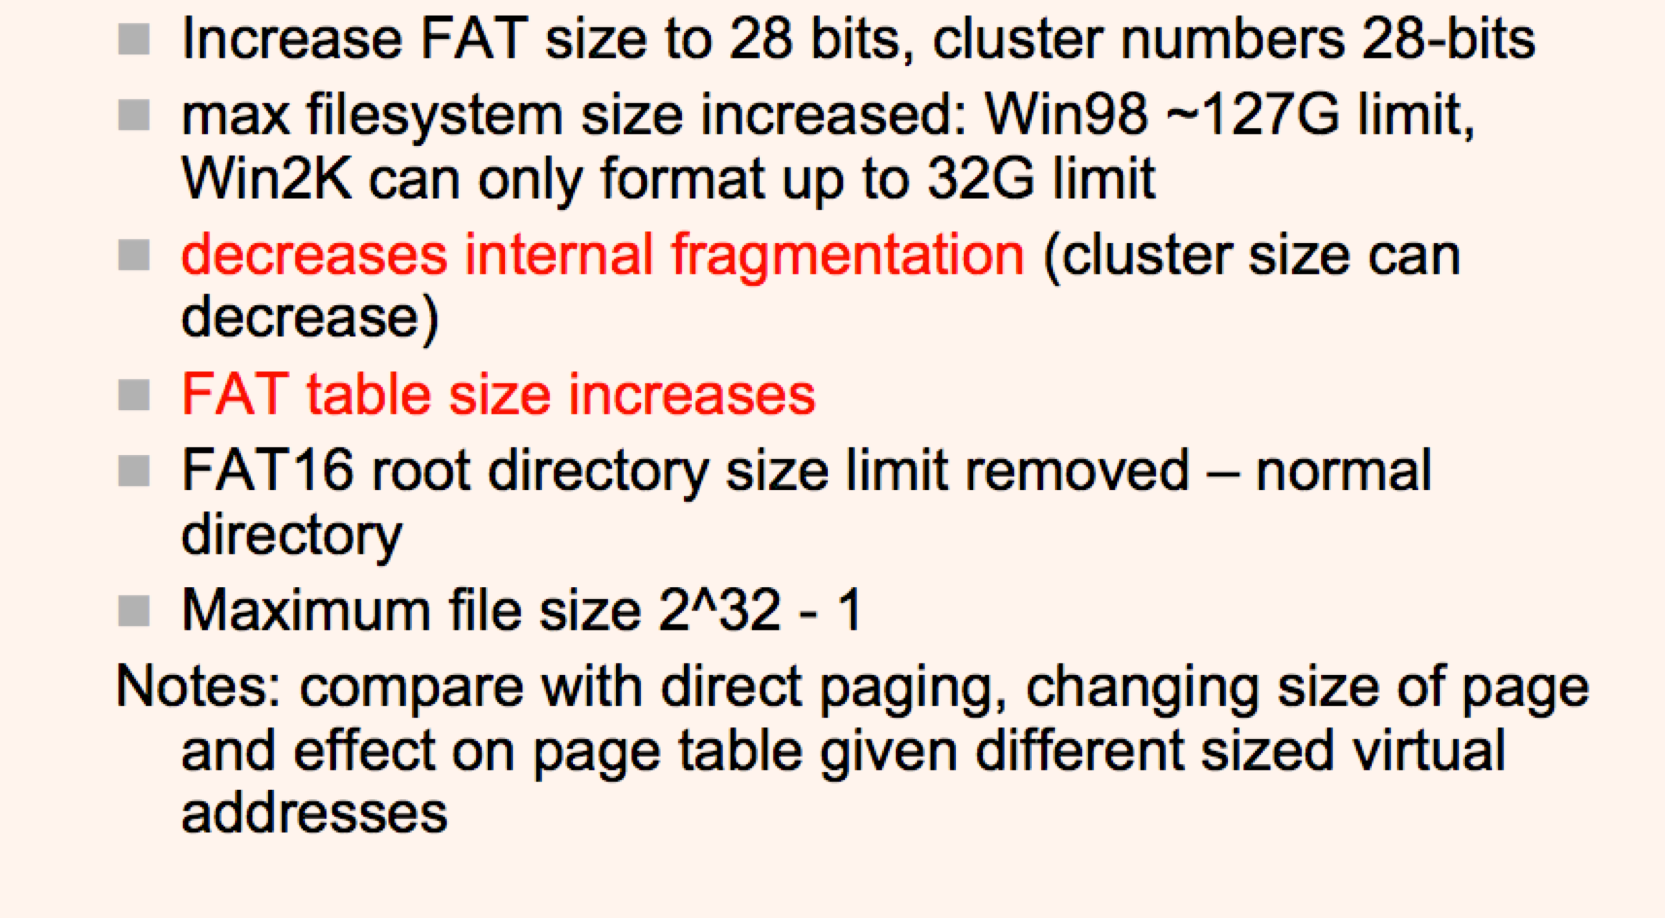
\includegraphics[width=0.50\linewidth]{m2/MSDOSFAT9}
			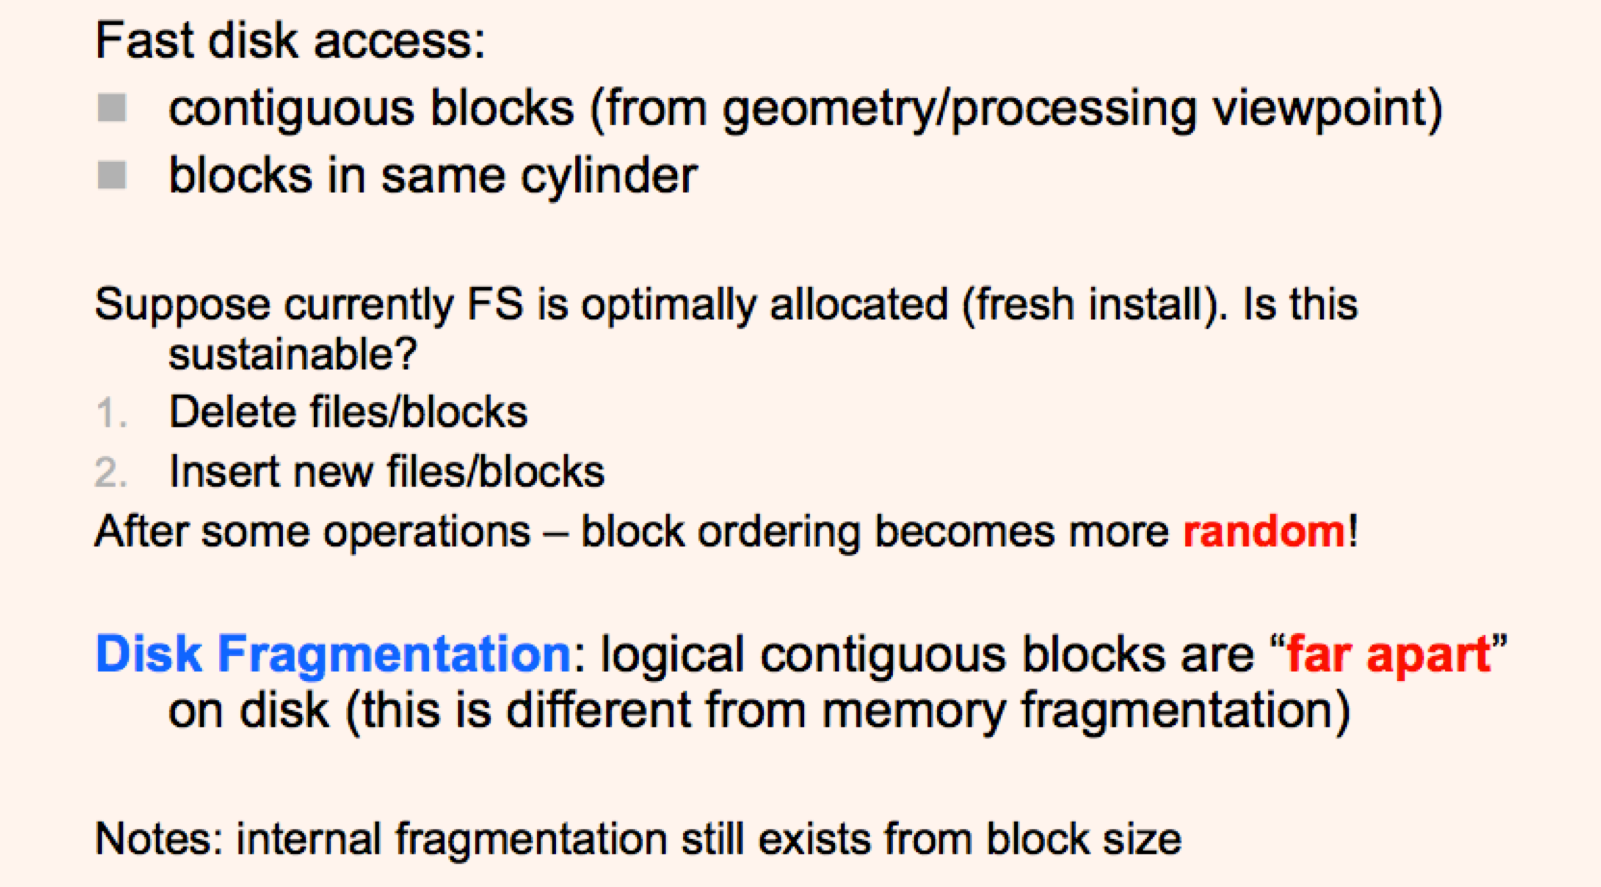
\includegraphics[width=0.50\linewidth]{m2/MSDOSFAT10}
			\begin{center}
				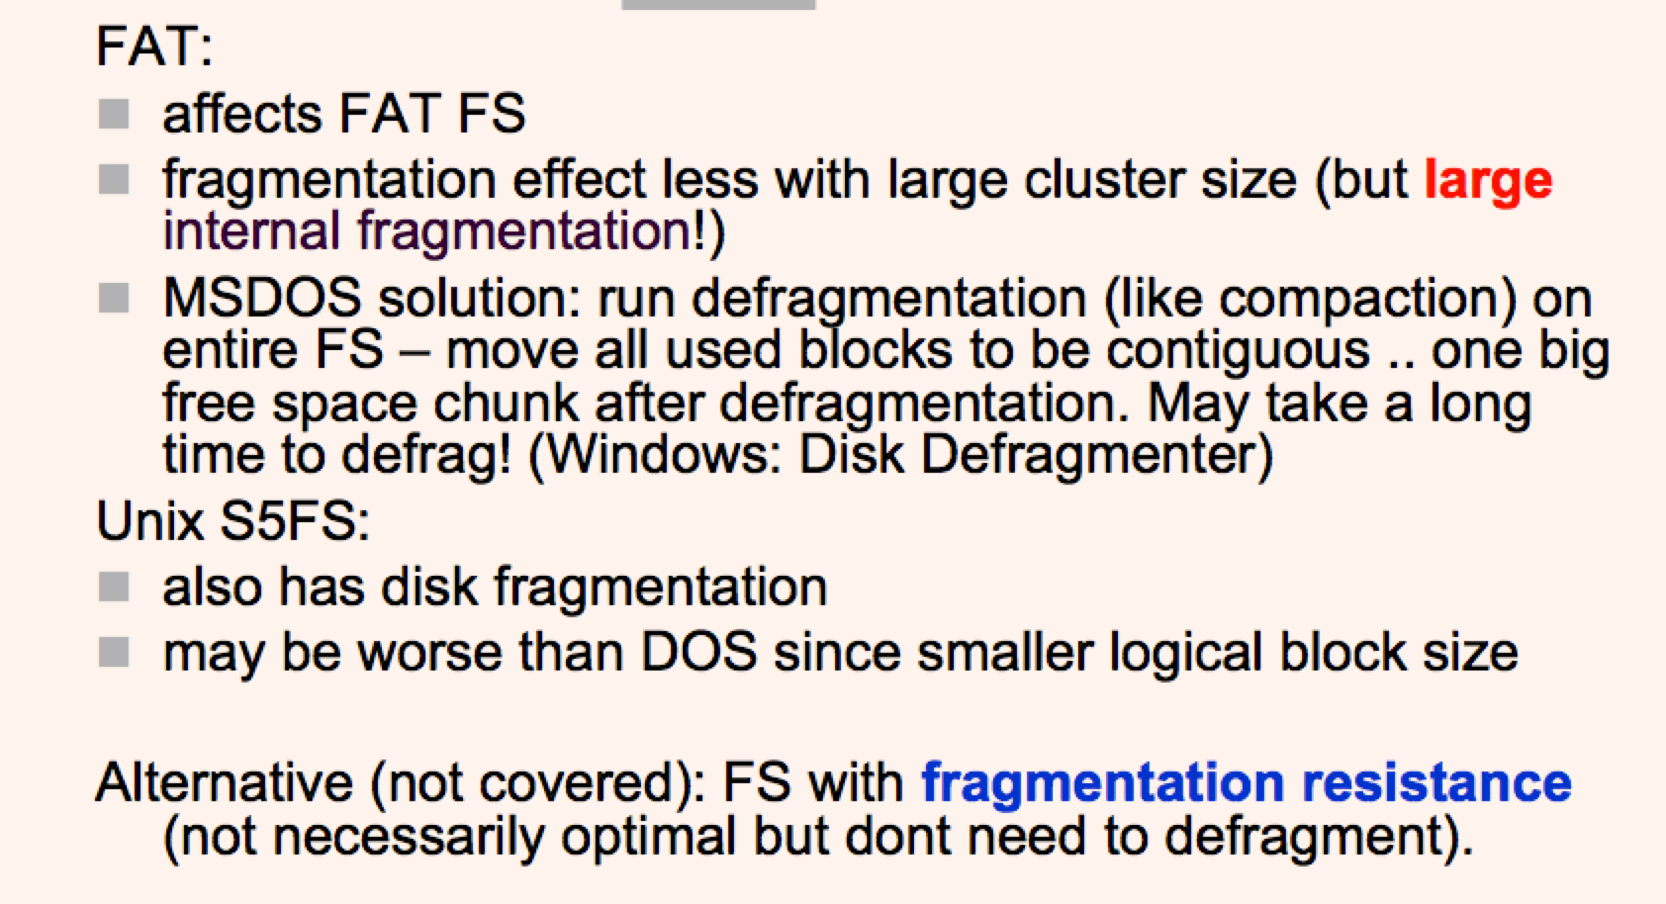
\includegraphics[width=0.50\linewidth]{m2/MSDOSFAT11}
			\end{center}
		\end{myenumerate}
		
		\item \textbf{Indexed organization}
		\begin{myenumerate}
			\item \textbf{Index table}: sequential list of records; \textbf{implementation}: keep index list in descriptor 
			\item \textbf{Advantage}: Insert/delete is easy; Sequential and direct access is efficient
			\item \textbf{Disadvantage}: file size limited by number of index entries
			
			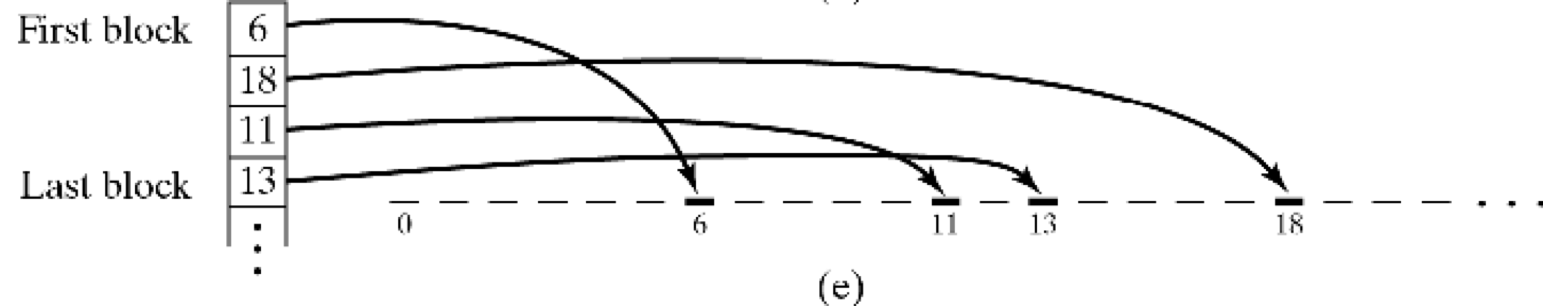
\includegraphics[width=1.0\linewidth]{m2/indexedOrganization}
			
			\item \textbf{Multi-level index hierarchy}: Primary index points to secondary indices \textbf{Problem}: number of disk accesses increases with depth of hierarchy.
			\item \textbf{Incremental indexing}: number of disk accesses increases with depth of hierarchy; When insufficient, allocate additional index levels; \textbf{Example}: Unix, 3-level expansion.
			
			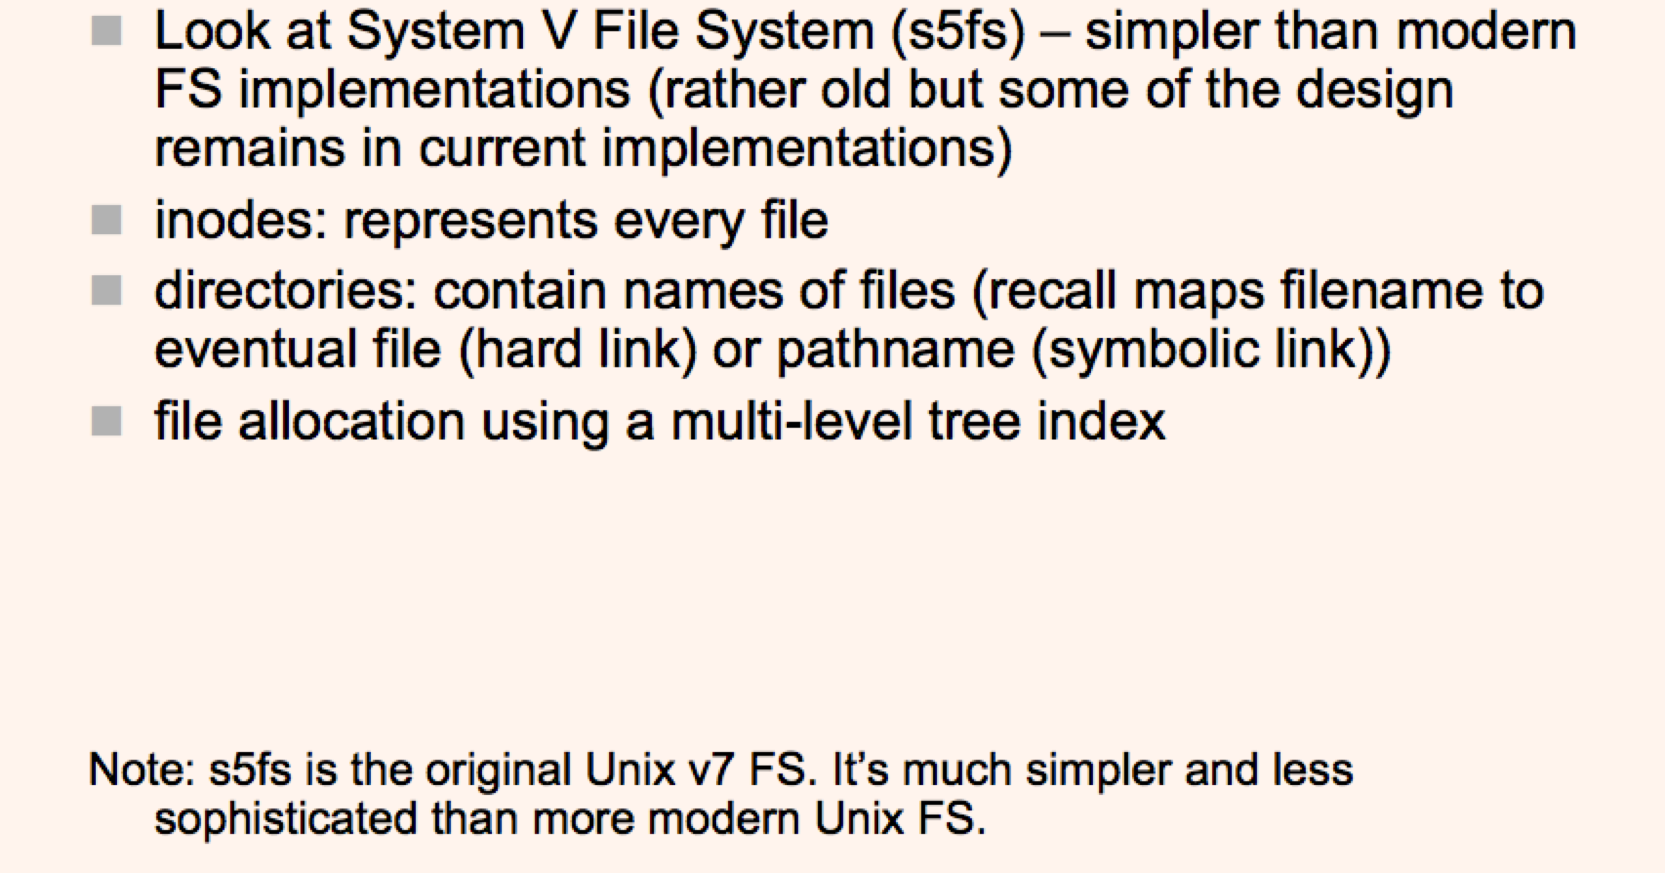
\includegraphics[width=0.50\linewidth]{m2/systemVFileSystem1}
			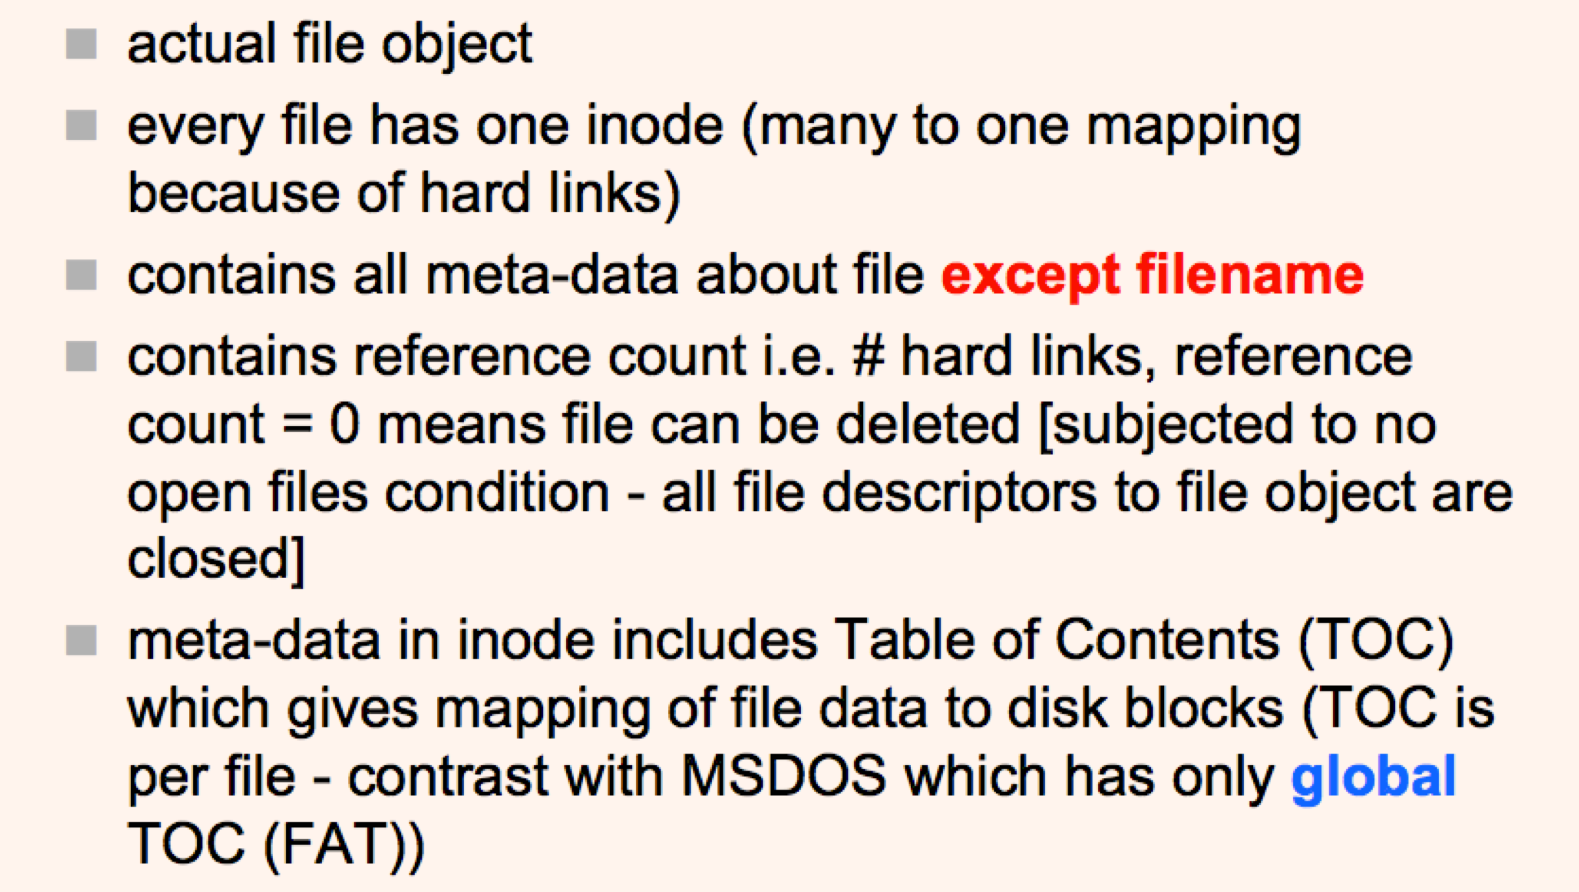
\includegraphics[width=0.50\linewidth]{m2/systemVFileSystem2}
			
			\begin{minipage}{0.5\linewidth}
				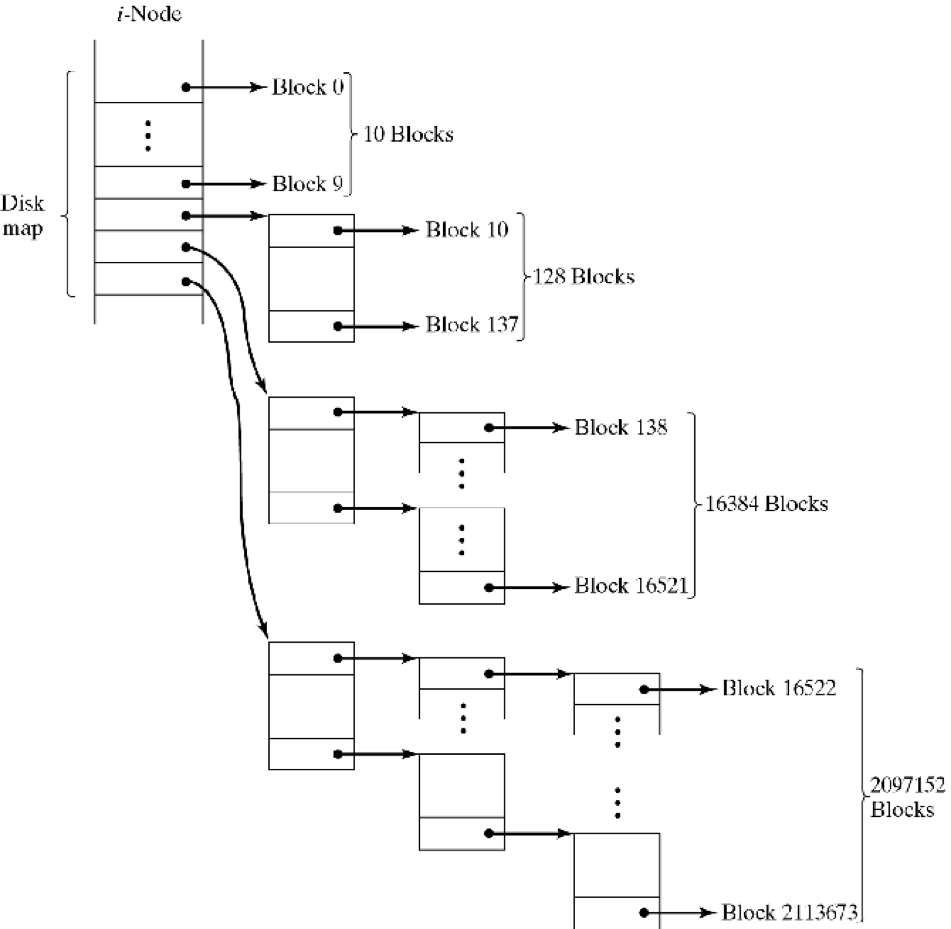
\includegraphics[width=1.0\linewidth]{m2/systemVFileSystem3}
			\end{minipage}
			\begin{minipage}{0.5\linewidth}
				\textbf{Incremental indexing in Unix} (file size vs. speed of access)
				\begin{myitemize}
					\item blocks 0-9: 1 access (direct).
					\item blocks 10-137: 2 access.
					\item blocks 138-16521: 3 access. etc.
				\end{myitemize}
				
				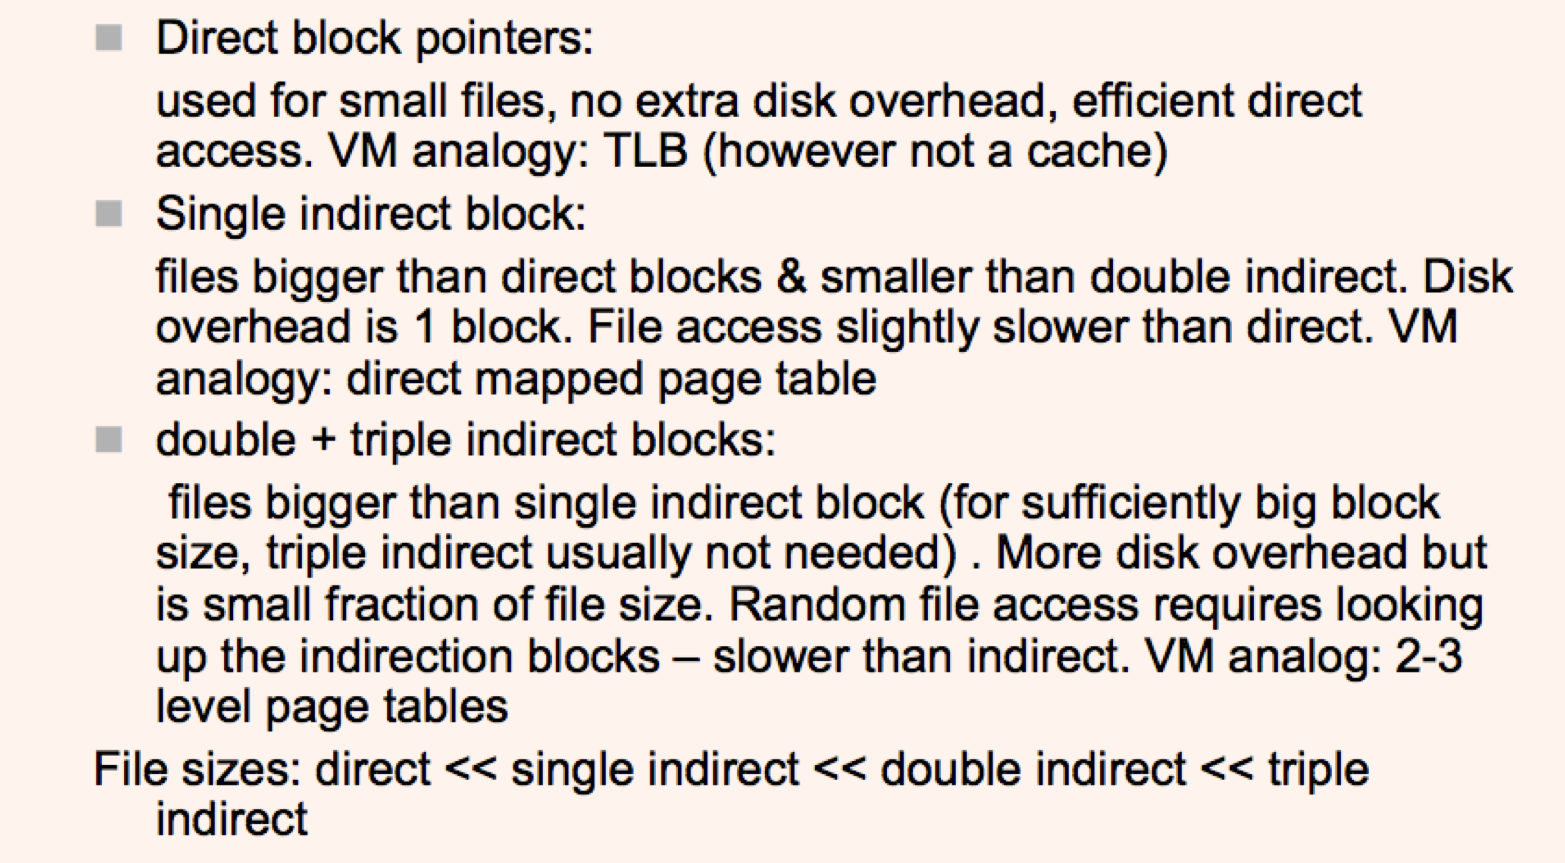
\includegraphics[width=1.0\linewidth]{m2/systemVFileSystem4}
			\end{minipage}
			
			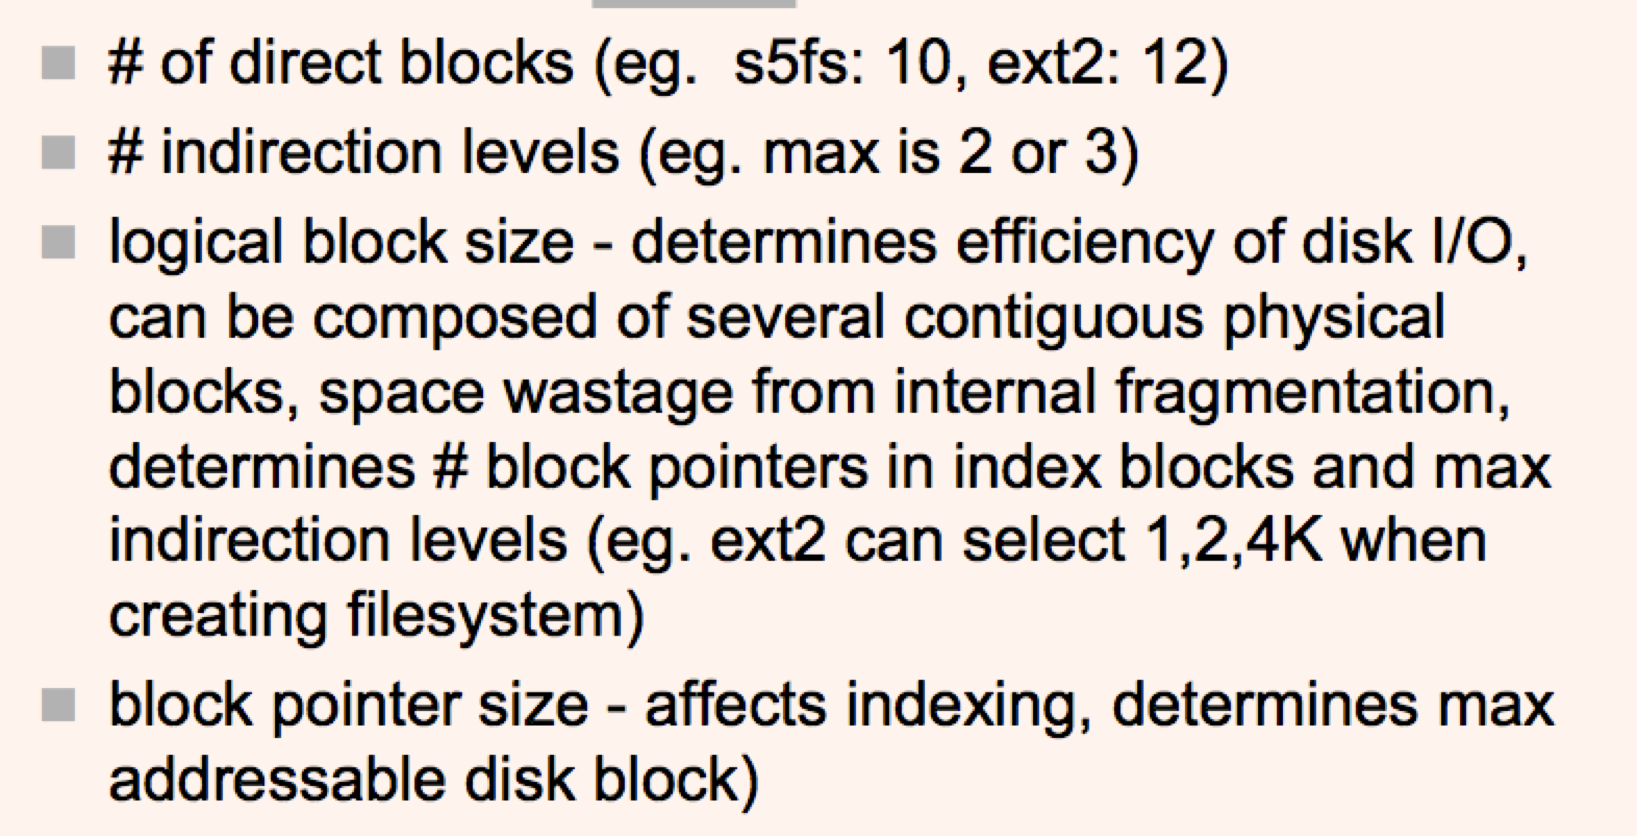
\includegraphics[width=0.50\linewidth]{m2/systemVFileSystem5}
			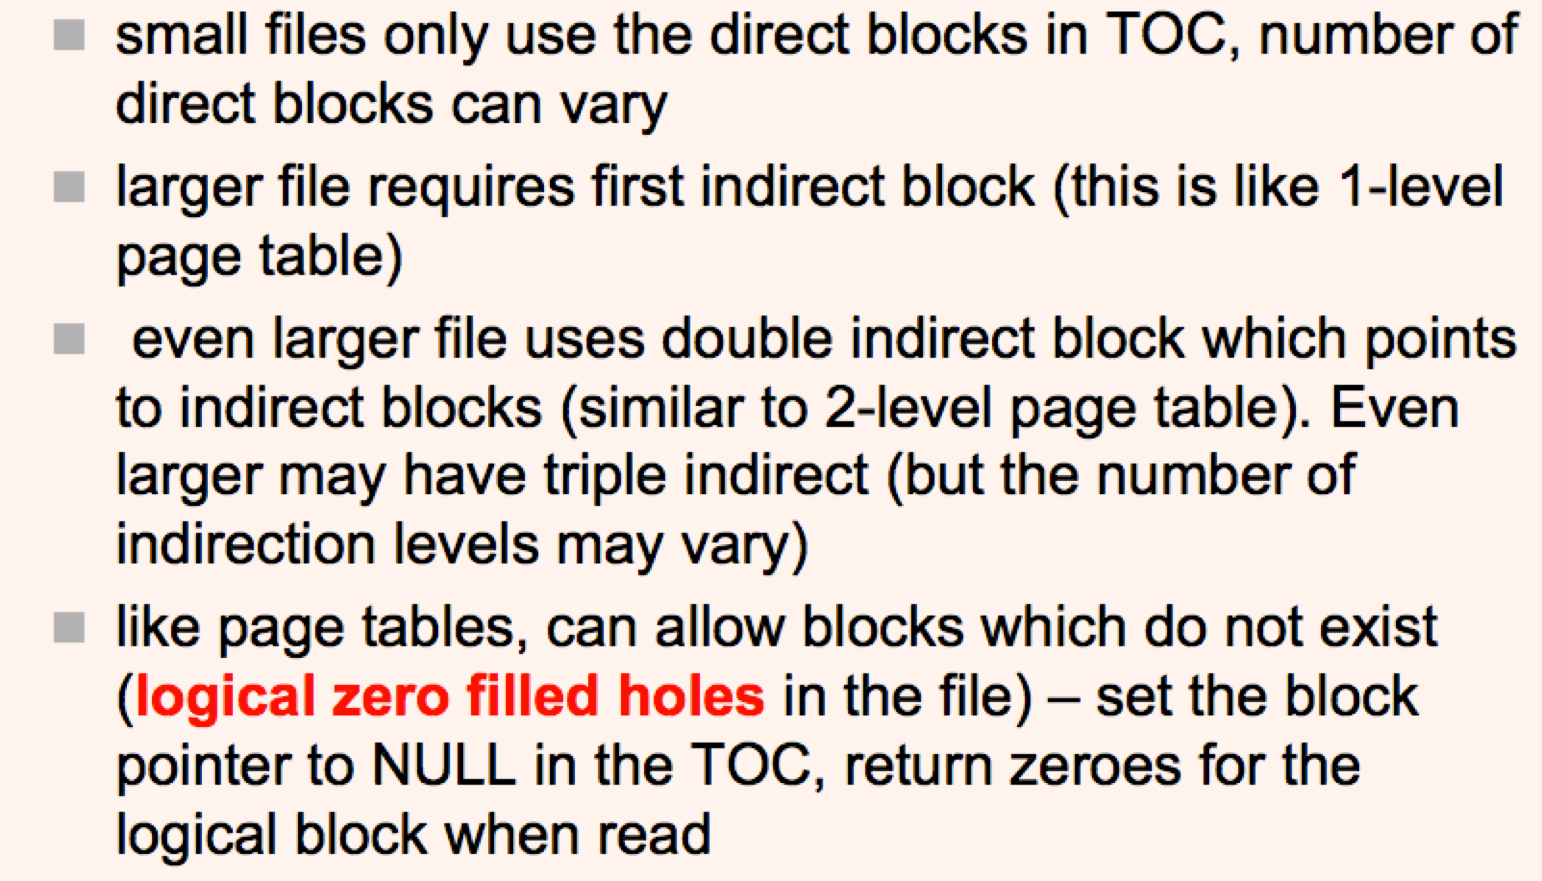
\includegraphics[width=0.50\linewidth]{m2/systemVFileSystem6}
			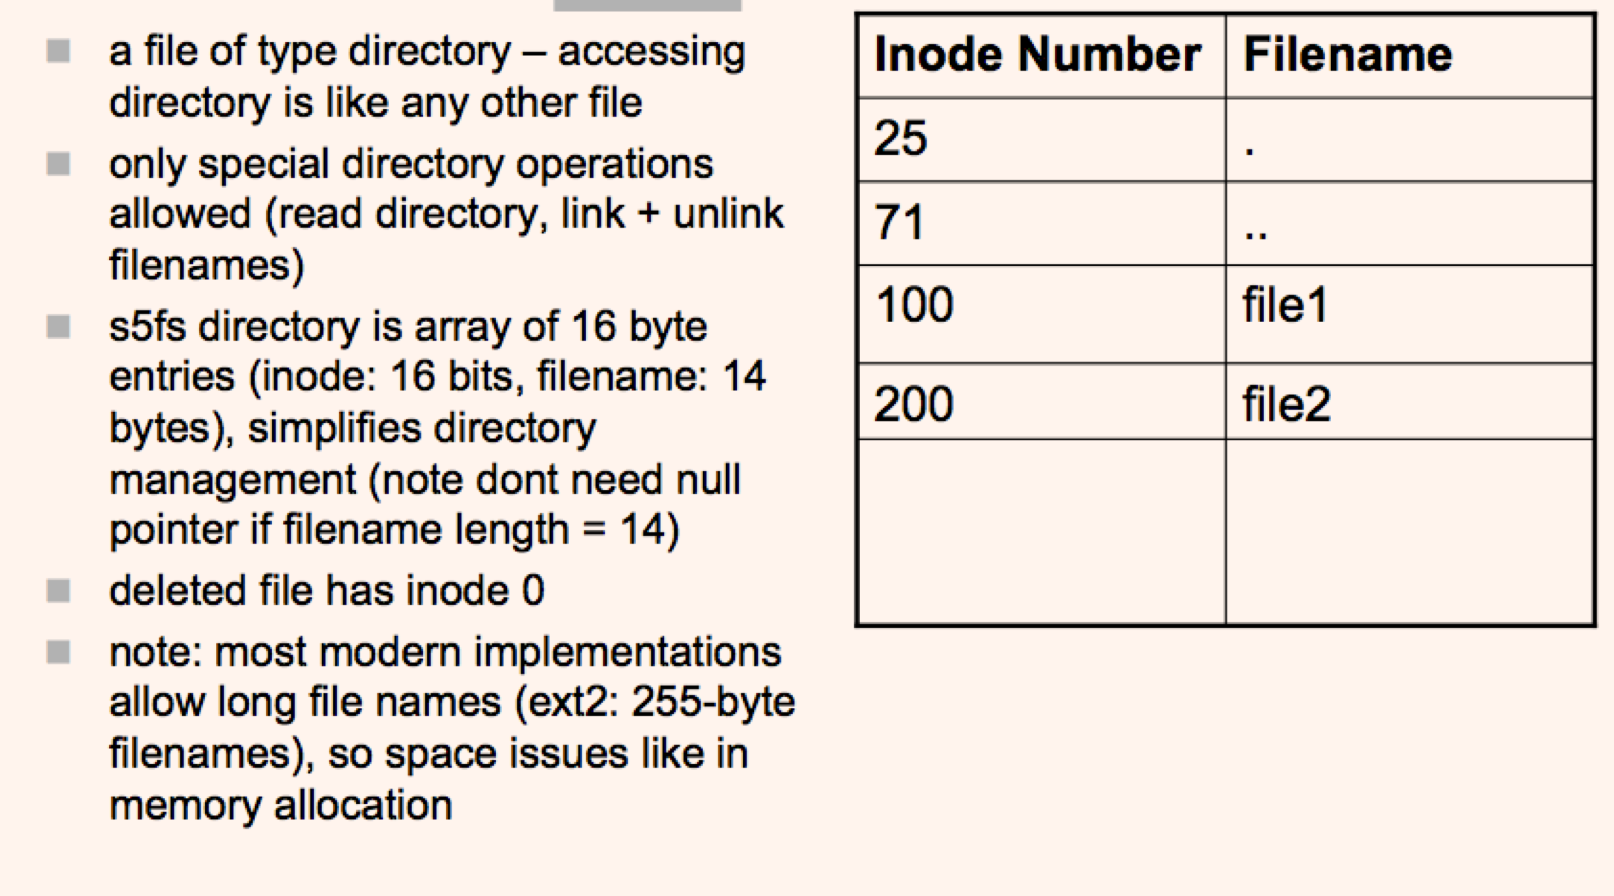
\includegraphics[width=0.50\linewidth]{m2/systemVFileSystem7}
			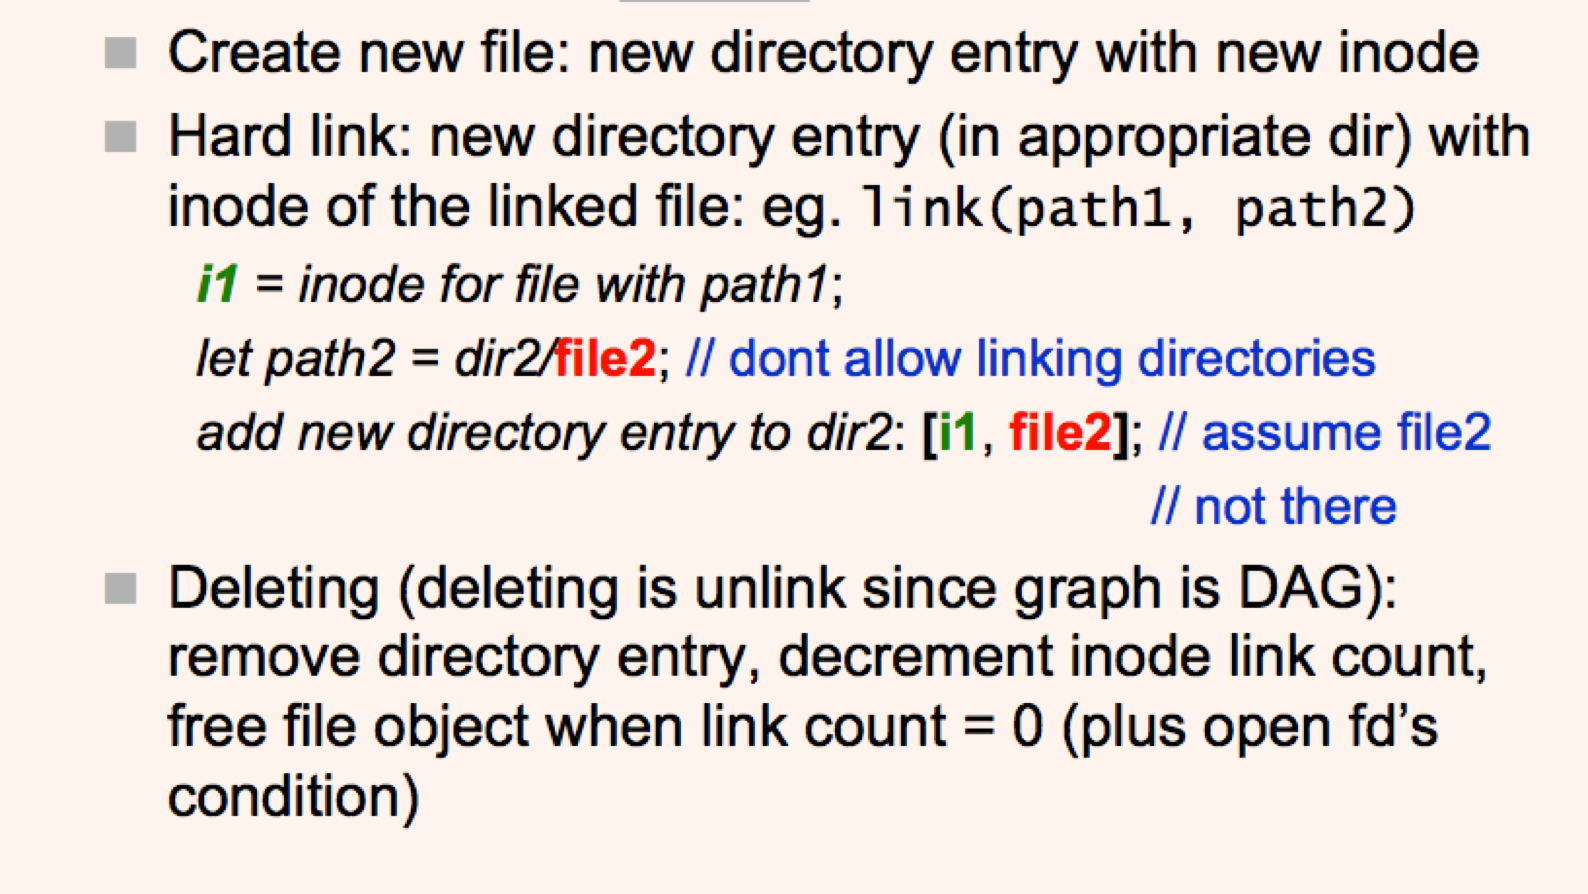
\includegraphics[width=0.50\linewidth]{m2/systemVFileSystem8}
		\end{myenumerate}
	\end{myitemize}
\end{definition}

\begin{definition}{\textbf{Free storage space management}}
	\begin{myitemize}
		\item \textbf{Linked list organization}
		\begin{myenumerate}
			\item Linking \textbf{individual} blocks: inefficient; no blocks clustering to minimise seek operations; groups of blocks are allocated/released one at a time.
			\item Better: Link \textbf{groups} of consecutive blocks
		\end{myenumerate}
		\item \textbf{Bit map organization}
		\begin{myenumerate}
			\item Analogous to main memory
			\item A single bit per block indicating if free or occupied
		\end{myenumerate}
	\end{myitemize}
\end{definition}

% $$$$$$$$$$$$$$$$$$$$$$$$$$$$$$$$$$ %
\end{document}